% !TeX encoding = UTF-8
% !TeX program = xelatex
% !TeX spellcheck = en_US

\documentclass[bachelor,arabic,pdf]{ustcthesis}
% doctor|master|bachelor [academic|professional] [chinese|english] [print|pdf]
% [super|numebers|authoryear]

\title{面向移动服务机器人的行人追踪跟随的研究与实现}
\author{韦清}
\major{计算机科学与技术}
\supervisor{陈小平\ 教授}
% \cosupervisor{钱学森\ 教授}
% \date{二〇一七年五月一日} % 注释掉则为今日
% \professionaltype{专业学位类型}
% \secretlevel{秘密}        % 绝密|机密|秘密,注释本行则不保密
% \secretyear{20}           % 保密年限

\entitle{Research and Implementation of People Tracking and Following with Mobile Service Robots}
\enauthor{Qing Wei}
\enmajor{Computer Science and Technology}
\ensupervisor{Prof. Xiaoping Chen}


% \encosupervisor{Prof. Xuesen Qian}
% \endate{May 1, 2017}      % Today if commented
% \enprofessionaltype{Professional degree type}
% \ensecretlevel{Secret}    % Top secret|Highly secret|Secret


% 加载宏包和配置
\usepackage{graphicx}
\graphicspath{{figures/}}
\usepackage{booktabs}
\usepackage{longtable}
\usepackage[ruled,linesnumbered]{algorithm2e}
\usepackage{siunitx}
\usepackage{amsthm}
\usepackage{hyperref}

\DeclareRobustCommand\cs[1]{\texttt{\char`\\#1}}
\newcommand\pkg{\textsf}

\renewcommand\vec{\symbf}
\newcommand\mat{\symbf}
\newcommand\ts{\symbfsf}
\newcommand\real{\mathbf{R}}




\begin{document}

% 研究生论文:
%   封面,原创性声明和授权使用声明
%   frontmatter: 摘要,目录,[图、表清单],[符号说明]
%   mainmatter: 正文章节,参考文献
%   appendix: 附录
%   backmatter: 致谢,已发表论文列表
%
% 本科生论文:
%   封面
%   frontmatter: 致谢,目录,摘要
%   mainmatter: 正文章节,参考文献
%   appendix: 附录

\maketitle
\makestatement

\frontmatter
\tableofcontents
% !TeX root = ../main.tex

\begin{abstract}
  服务机器人是一种能完成有益于人类的服务工作的半自助或全自主型机器人,分为个人/家庭服务机器人和专业机器人。专业机器人一般在特定场景中使用,如商业服务、物流、医疗、救援等;而个人/家用服务机器人主要在日常生活场景中进行与人进行交互,提供家政服务、陪伴、娱乐、辅助学习等多种功能,包括家政机器人、娱乐休闲机器人、助老助残机器人等。其中,个人/家庭服务机器人为本文研究内容所适用的对象。

  随着人工智能与物联网技术迅速发展,个人家庭用机器人、公共服务机器人的应用场景、服务模式和市场也在不断拓展,成为了当下的一个研究热点。为了精准理解当前环境和有效执行指令,能够精确可靠地自动识别目标人物并对其进行追踪陪同,是这类移动服务机器人的人机交互中的一项重要且必要的功能。

  本文将针对室内移动机器人的行人跟随问题做如下三个方面的研究:

  (1)常用目标跟随算法的原理与实现:主要从行人检测和追踪两个角度进行调研论述。主要介绍了用于行人检测的几个常用特征,如颜色直方图、LBP、HOG、SIFT特征,基于机器学习的几种分类器,包括KNN、SVM、RandomForest、AdaBoost,以及几种常用的追踪算法,包括卡尔曼滤波、粒子滤波、均值漂移、相关滤波等。

  (2)ROS上的机器人导航技术;主要包括ROS提供的ROS导航包,以及中科大研发的可佳机器人的导航功能。

  (3)可佳机器人上行人跟随系统的实现;结合行人的HOG特征和HSV直方图特征,使用CSR-DCF算法进行行人追踪,并单独训练一个SVM分类器以防止追踪器发生误判/漏判,以及帮助追踪器从追踪失败中恢复。

  \keywords{计算机视觉;机器人;行人检测;目标追踪}
\end{abstract}

\begin{enabstract}
  A service robot is a robot which operates semi- or fully autonomously to perform services useful to the well-being of humans and equipment. They are capable of making decisions and acting autonomously in real and unpredictable environments to accomplish determined tasks.  There are two types of service robots, personal/domestic service robots and professional robots. Professional robots are typically used in specific occasions, including business, delivery, medical, rescue, etc. Personal/domestic service robots, which include cleaning robots, elder care and medical companions, entertainment and leisure robots, home education and training robots, are the specific application objects of the research in this paper.

  With the rapid development of artificial intelligence and IOT, the application scenarios, service patterns and market of service robots are also continuously expanding, thus making the service robots a focused area in Robotics research. In order to accurately understand the current environment and effectively execute the instructions, one of the important and necessary ability for a personal service robot, is to automatically recognize and track a person precisely and robustly.

  This paper is consist of three parts:

  (1) The theories and implementation of various existing object tracking algorithm;

  (2) Robot navigation on ROS;

  (3) The implementation of the people following system on kejia robot.

  \enkeywords{Computer Vision; Robotics; Pedestrian Detection; Object Tracking}
\end{enabstract}
% \listoffigures
% \listoftables
%% !TeX root = ../main.tex

\begin{notation}

  \begin{notationlist}{2em}
    \item[$\displaystyle a$] The number of angels per unit area
    \item[$\displaystyle N$] The number of angels per needle point
    \item[$\displaystyle A$] The area of the needle point
    \item[$\displaystyle \sigma$] The total mass of angels per unit area
    \item[$\displaystyle m$] The mass of one angel
    \item[$\displaystyle \sum_{i=1}^n a_i$] The sum of $a_i$
  \end{notationlist}

\end{notation}



% 也可以使用 nomencl 宏包

% \printnomenclature

% \nomenclature{$\displaystyle a$}{The number of angels per unit are}
% \nomenclature{$\displaystyle N$}{The number of angels per needle point}
% \nomenclature{$\displaystyle A$}{The area of the needle point}
% \nomenclature{$\displaystyle \sigma$}{The total mass of angels per unit area}
% \nomenclature{$\displaystyle m$}{The mass of one angel}
% \nomenclature{$\displaystyle \sum_{i=1}^n a_i$}{The sum of $a_i$}


\mainmatter
% !TeX root = ../main.tex

\chapter{绪论}

\section{研究背景及意义}

  服务机器人是一种半自助或全自主工作的机器人。它能完成有益于人类健康的服务工作,但不包括从事生产的设备。它们可以在真实且不可预测的环境中自动进行决策和行动来完成确定的任务。服务机器人分为个人/家庭服务机器人和专业机器人。专业机器人一般在特定场景中使用,如商业服务、物流、医疗、救援等;而个人/家用服务机器人主要在日常生活场景中进行与人进行交互,提供家政服务、陪伴、娱乐、辅助学习等多种功能,包括家政机器人、娱乐休闲机器人、助老助残机器人等。其中,个人/家庭服务机器人为本文研究内容的应用对象。

  随着人工智能与物联网技术不断发展,服务机器人作为智能硬件之一,不断地丰富其自身功能及其实现更强大的性能,服务机器人市场也在迅速发展,家庭用机器人、智能公共服务机器人的应用场景和服务模式不断拓展。为了精准理解当前环境和有效执行指令,能够精确可靠地自动识别目标人物并对其进行追踪陪同,是这类移动服务机器人的人机交互中的一项重要且必要的功能。这项功能可以用于在博物馆或医院等场景中对用户进行指引,在家庭中陪伴用户、与用户进行交互,助老、助残等。

  移动机器人的核心技术包括导航定位、地图创建、路径规划、任务分配和目标跟踪等。在本文中,会主要介绍目标跟踪,尤其是其中的行人定位模块,通过对ROS导航的简要介绍涉及机器人导航定位、地图创建、路径规划的大致概念,并最终实现一个有简单导航模块和较为鲁棒的行人追踪模块的机器人系统。

\section{相关工作}

  自从有了服务机器人的概念以来,就有了很多对于机器人目标跟随技术的研究。移动机器人由于可携带多种传感器,由此衍生了各种使用了传感器的行人识别和追踪方法。如使用视觉图像、激光传感器、热成像传感器\cite{treptow2006real}、声音传感器\cite{zhou2008target}等,由于单一传感器信息较少,也出现了不少多传感器融合的行人定位方式\cite{susperregi2013rgb}。

  激光传感器由于还被广泛运用到机器人的定位、建图、导航中,是机器人最为重要的传感器,所以也最多地被运用到行人跟随的任务中。不过激光传感器由于成本限制,多使用2D激光检测同一水平面的物体,竖直空间上可以检测到的范围有限,所以激光行人追踪的方法最为经常使用的特征是行人的双腿\cite{arras2008efficient}。在激光图像中,人的双腿在有一种明显的模式,通过滤波器抽取人的腿部特征,进行聚类,便可得到一个人腿模式识别器,再结合粒子滤波或卡尔曼滤波等技术,便可以实现对行人腿部的持续追踪。但这种识别器在有遮挡时,或暂时失去目标后,无法准确地重新建立对目标的追踪。此外,从人腿信息中基本不可能对不同行人加以区分,所以为了系统的鲁棒性,行人腿部识别通常还是需要加入视觉信息,如结合面部识别,来进行一些情况下的行人的区分\cite{kleinehagenbrock2002person,bellotto2008multisensor}。

  视觉行人追踪中也有很多已有的方法,包括对行人的面部识别\cite{wong1995mobile,cruz2008rea}(要求行人必须面对相机),衣着识别\cite{bellotto2008multimodal,noceti2009combined}(主要通过对衣着颜色特征的提取),身体轮廓识别\cite{}(使用HOG、边缘描述子等特征),行人步态识别\cite{mowbray2003automatic,koide2016identification}等。

  但在现有的大多行人追踪算法中也存在一些问题,如在行人在视野中消失或被遮挡一段时间后,追踪器如何从失败中恢复。本文在接下来会对行人检测和追踪常用的特征进行分析,选择合适的特征和追踪器实现一个视觉行人追踪系统,并尝试解决追踪器丢失目标后的恢复问题。



% !TeX root = ../main.tex

\chapter{行人追踪算法}
  
\section{视觉行人追踪}
  计算机视觉中的行人追踪,主要包括密集跟踪方法,即基于行人检测和识别的追踪,以及稀疏跟踪方法,即基于目标动态的追踪。

  在密集跟踪方法中,我们实际上并没有“跟踪”物体,而是在视频不同的时间点的一系列帧上扫描和检测物体的位置。由于每次的目标检测都是独立地在当前帧上进行的,所以每次检测时,都需要处理图像中的所有像素,所以以这种方法进行目标跟踪,计算量会比较大。

  由于目标的运动通常是连续的,稀疏跟踪方法即根据物体的动态信息,对其可能的运动轨迹进行预测,并结合其上一帧所在位置和对当前帧的观察,得出其当前位置的算法。由于已知物体在上一帧时的位置,所以对当前帧识别时,只需要检测上一帧物体所在位置附近的像素,这样一来,相对于密集跟踪方法,就减少了大量的计算。此外,由于我们结合了对物体运动的预测和观察来进行估计,在一些情况下准确度也会较高,此外,当物体被暂时遮挡时,目标检测在此时很大可能下会直接失败,但由于在追踪时我们还记录了物体最后出现的位置和对其行为的预测,所以可以在一定准确程度上继续追踪物体。但在物体速度较快时,可能会失去对物体的追踪,当目标物暂时从视野中消失一段时间时,可能难以重新找回物体。

  下面主要介绍在每帧上的行人检测,和以此为基础的动态行人追踪。

\subsection{行人检测}

  经典的基于检测的追踪方法包括提取人工特征,在使用分类器进行分类,分类器包括支持向量机(Support Vector Machines, SVM),随机森林分类器(Random Forest)和各种Boosting算法(如AdaBoost)。

\subsubsection{常用特征描述子}

  特征描述子是一种对图片的表示方法,它通过提取图片中的关键信息并丢弃多余信息来对图片信息进行简化。通常地,特征描述子将一个RGB三通道的图片转化成一个特征向量。
  
  为了做到精确地进行图像识别、目标检测,我们必须首先明确什么是关键的、有用的信息,什么是冗余信息。

\paragraph{颜色直方图}

  颜色特征具有旋转不变性,且不受目标的大小和形状的变化影响,在颜色空间中分布大致相同,从而具有较高的鲁棒性。

  颜色直方图是描述颜色特征最常用的描述子,它是是对目标表面颜色分布的统计,描述了不同色彩在图像中所占的比例,但无法描述图像中颜色的局部分布及每种色彩所处的空间位置,即无法描述图像中的某一具体的对象或物体。颜色直方图具有稳定性好、抗部分遮挡、计算方法简单和计算量小的特点。

  颜色直方图可以基于不同的的颜色空间,其中,最常用的是RGB空间和HSV空间。以RGB空间为例,分别统计每个像素的R、G、B数值落在[0,255]上每个点的频度,绘制出直方图,该图片的颜色特征即为三个长为256的向量,分别表示其的红色、绿色、蓝色的统计分布。以一张人物照片\ref{fig:ewan}为例,图\ref{fig:rgbhistogram}为其RGB颜色直方图。

\begin{figure}[htb]
  \centering
  
\includegraphics[width=0.3\textwidth]{ewan.jpg}
  \caption{原图}
  \label{fig:ewan}
\end{figure}

\begin{figure}[htb]
  \centering
  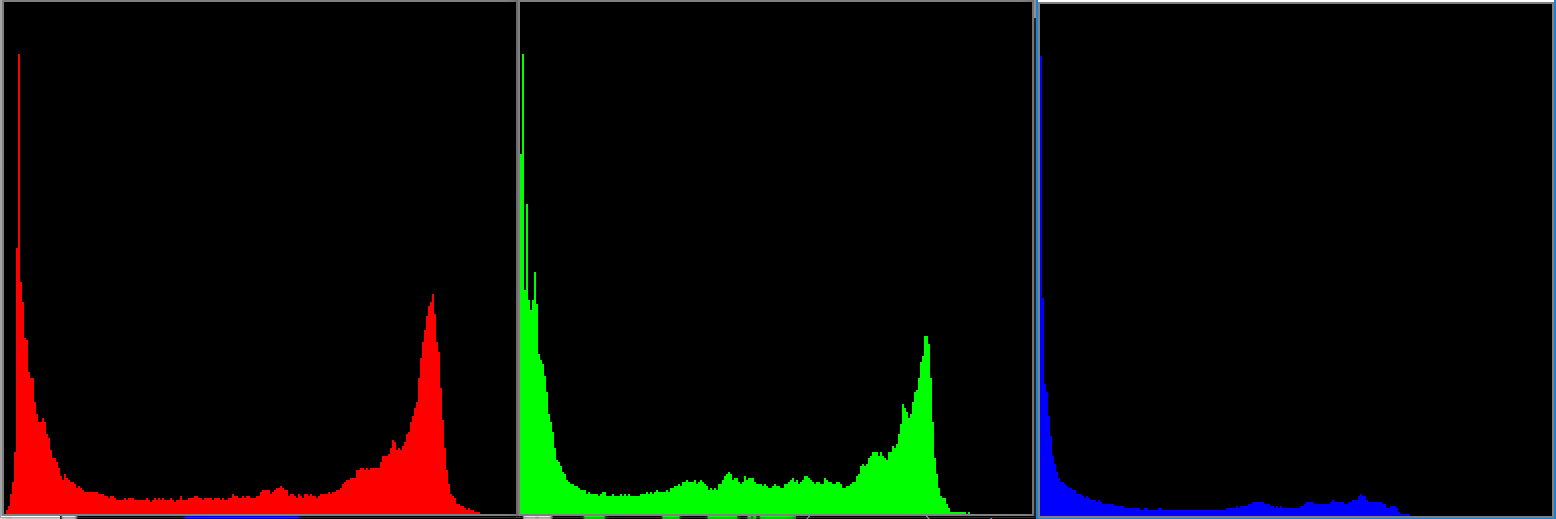
\includegraphics[width=0.6\textwidth]{rgb_histogram.png}
  \caption{左:B通道颜色直方图;中:G通道颜色直方图;右:R通道颜色直方图}
  \label{fig:rgbhistogram}
\end{figure}

  但RGB颜色空间的均匀性非常差,且两种颜色之间的直觉差异色差不能表示为改颜色空间中两点间的距离,RGB这三种颜色的分量的取值与所生成的颜色之间的联系并不直观。

  在计算机视觉中,我们常采用HSV颜色空间来表示颜色。HSV是一种将RGB色彩空间中的点在圆柱坐标系中的表示方法,相对于RGB,它能够更加直观地表示色彩的明暗、色调以及鲜艳程度,方便进行颜色之间的对比。此外,由于HSV单独提取了颜色的明暗,也可以一定程度上抵抗光照明暗带来的影响。\citet{sural2002segmentation}的实验显示,使用HSV直方图进行行人识别的结果相比RGB直方图有了明显提高。

  HSV即色相(Hue)、饱和度(Saturation)、亮度(Value)。色相即表示物体的颜色,如红色、黄色等,在$0^{\circ}$到$360^{\circ}$的标准色轮上,按位置度量色相;饱和度是指颜色的强度或纯度,表示色相中灰色分量所占的比例,它使用从0\%(灰色)至100\%(完全饱和)的百分比来度量;亮度是颜色的相对明暗程度,通常使用从0\%(黑色)至100\%(白色)的百分比来衡量。

\begin{figure}[htb]
  \centering
  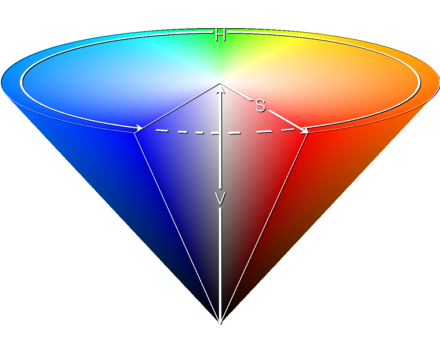
\includegraphics[width=0.3\textwidth]{hsv.png}
  \caption{HSV模型可以使用圆柱坐标系中的一个圆锥形子集表示}
  \label{fig:hsv}
\end{figure}

  由于大部分数字图像都是基于RGB空间进行表示的,我们需要首先把RGB空间坐标映射到HSV空间。给定$(r,g,b)$分别是一个颜色的红、绿、蓝坐标,它们的值是在0到1之间的实数,$max$为$r$,$g$和$b$之中的最大值,$min$为其中的最小值,则从$(r,g,b)$到$(h,s,v)$的转换公式如下:\cite{foley1982fundamentals}

$$h={\begin{cases}0^{\circ }&{\mbox{if }}max=min\\60^{\circ }\times {\frac  {g-b}{max-min}}+0^{\circ },&{\mbox{if }}max=r{\mbox{ and }}g\geq b\\60^{\circ }\times {\frac  {g-b}{max-min}}+360^{\circ },&{\mbox{if }}max=r{\mbox{ and }}g<b\\60^{\circ }\times {\frac  {b-r}{max-min}}+120^{\circ },&{\mbox{if }}max=g\\60^{\circ }\times {\frac  {r-g}{max-min}}+240^{\circ },&{\mbox{if }}max=b\end{cases}}$$

$$s={\begin{cases}0,&{\mbox{if }}max=0\\{\frac  {max-min}{max}}=1-{\frac  {min}{max}},&{\mbox{otherwise}}\end{cases}}$$

$$
v=max
$$

  HSV直方图的计算与RGB类似,只是将颜色空间有所差异,我们同样使用图片\ref{fig:ewan}计算其HSV直方图,见图\ref{fig:hsvhistogram}。

\begin{figure}[htb]
  \centering
  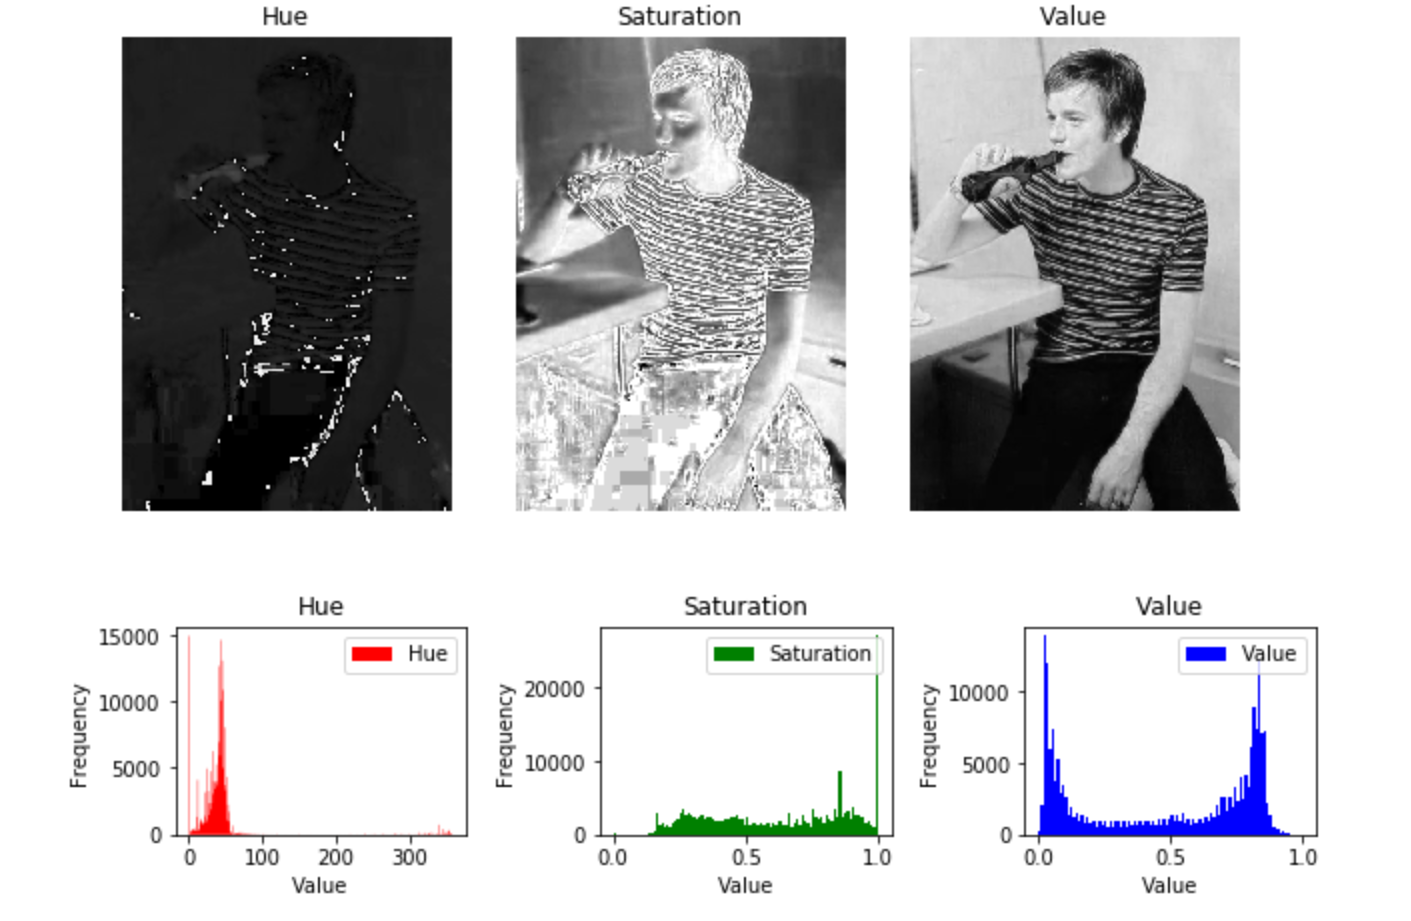
\includegraphics[width=1.0\textwidth]{hsv_histogram.png}
  \caption{左:H通道灰度图和颜色直方图;中:S通道灰度图和颜色直方图;右:V通道灰度图和颜色直方图}
  \label{fig:hsvhistogram}
\end{figure}

\paragraph{局部二值模式}

  局部二值模式(Local Binary Pattern,LBP)是一种用来描述图像局部纹理特征的特征描述子,具有旋转不变性和对光照变化不敏感等优点,由\citet{ojala1994performance}在1994年首次提出。

  LBP的计算方法非常简单。每个像素都根据它相邻的八个像素按规定的顺序(如顺时针、逆时针)作比较,来确定其特征值。对于中心像素大于某个相邻像素的,该像素对应的二进制位设置为0,否则设置为1,比较了中心点相邻的八个像素后,就得到了一个8位的二进制数,这个数字即为中心像素的特征值,如图\ref{fig:lbp_procedure}所示,将每个点的LBP值使用灰度图表示,得到LBP图谱如\ref{fig:lbp}为例。

\begin{figure}[htb]
  \centering
  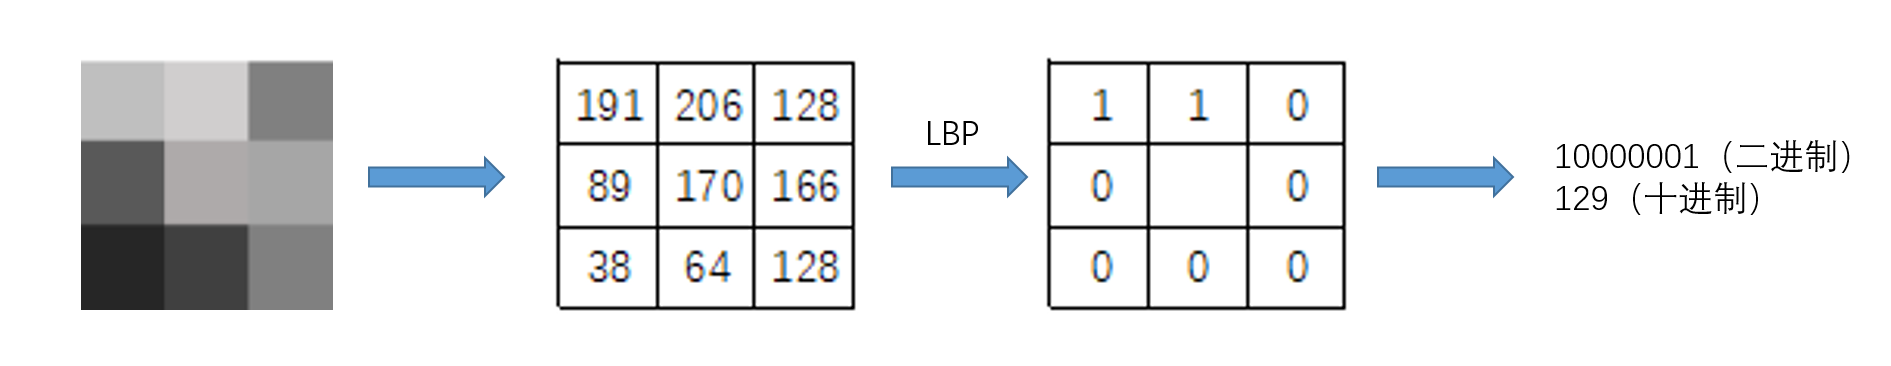
\includegraphics[width=0.9\textwidth]{LBP.png}
  \caption{计算3x3像素块中中心点的LBP值}
  \label{fig:lbp_procedure}
\end{figure}

\begin{figure}[htb]
  \centering
  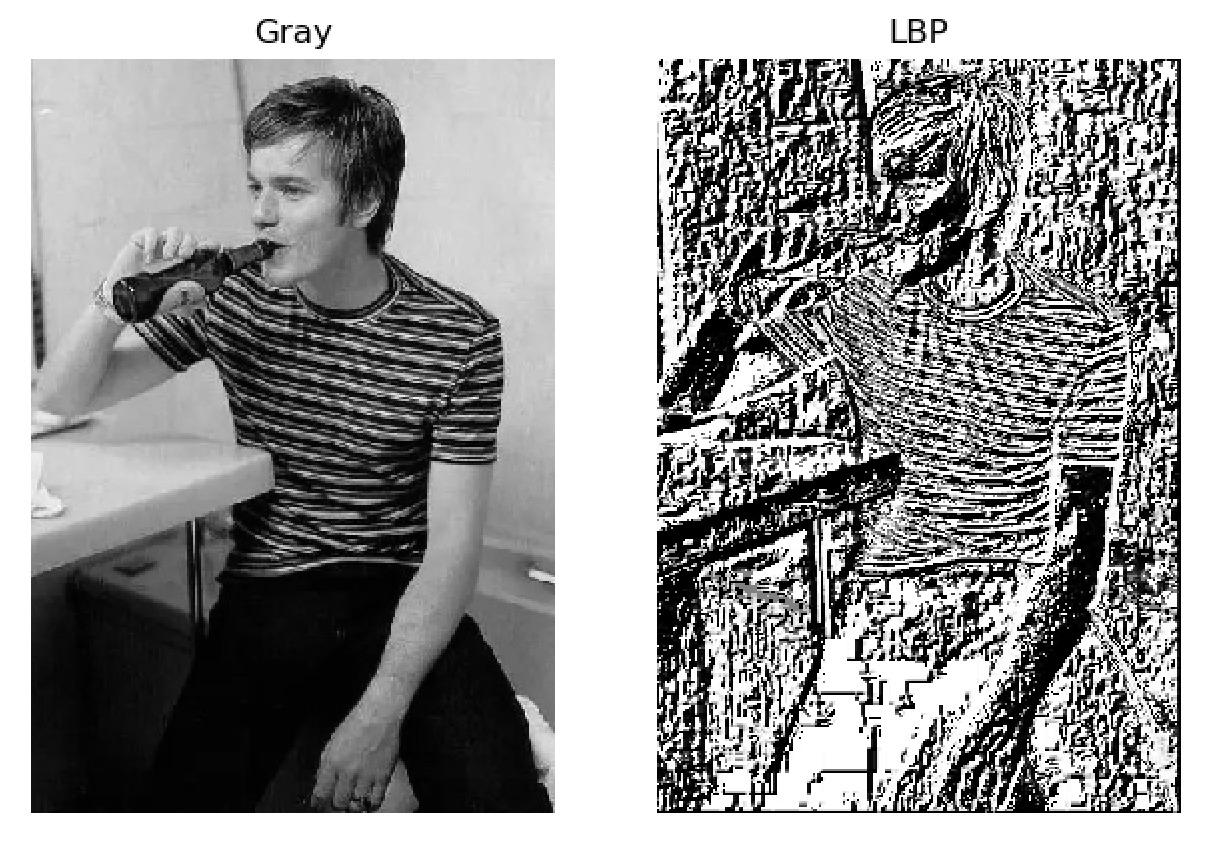
\includegraphics[width=0.6\textwidth]{ewan_lbp.png}
  \caption{左:灰度图;右:由灰度图计算得到的LBP图谱}
  \label{fig:lbp}
\end{figure}

  为了使得LBP描述子有旋转不变性,\citet{ojala2002multiresolution}提出了一个LBP的具有旋转不变性扩展方法,即不断旋转其邻域,得到一系列的LBP值,取其最小值作为该点的局部二值模式值。

  在计算一个图片的LBP描述子时,首先将图片分成固定大小的单元格(如$16\times16$像素),在计算出每个像素的LBP值后,统计每个单元格内的LBP值直方图,再串联所有单元格的直方图,即可得到该图片的LBP特征向量。

\paragraph{方向梯度直方图}

  方向梯度直方图(Histogram of Oriented Gradient, HOG)是目前行人识别中最广泛使用的特征描述子之一。\citet{dalal2005histograms}在2005年提出HOG结合SVM(支持向量机,support vector machine)进行行人检测的方法,在此之后,该方法被广泛应用到了图像识别中,并尤其在行人检测中获得了巨大的成功,也出现了很多改进和变体。

  在HOG特征描述符中,它通过计算和统计图像局部区域的梯度方向直方图来构成特征。由于在物体的边缘和角落处图片的颜色会进行突变,故在这些区域,梯度的大小会很大,显然,边缘和角落比起平坦区域包含更多关于物体形状的信息。而通过对边缘和角度的描述,HOG正可以很好地描述局部目标的表面质地和形状信息。但同时,由于梯度的性质,HOG特征描述字对噪点比较敏感,且由于HOG主要描述了物体的轮廓,所以很难处理遮挡问题。

  为了计算方向梯度,我们可以简单地使用内核(Kernel)$[-1,0,1]$和$[-1,0,1]^{T}$对原图进行过滤,分别得到横向和纵向上的有向梯度。除了这种方法之外,还可以使用$[-1,1],[1,-8,0,8,-1]$和Sobel算子等作为内核,不过根据\citet{dalal2005histograms}的实验,使用最简单的$[-1,0,1]$进行计算的梯度,在以HOG为特征进行的图像识别中效果最佳。

  在每个像素处,方向梯度都具有大小和方向。对于彩色图像,我们分别计算RGB三个通道的梯度。对原图片上的每个像素点$(x,y)$,$f(x,y)$为其R、G、B值中的一个,该通道上的横向和纵向方向梯度为:
\begin{gather*}
g_x(x,y)=[-1,0,1]\ast f(x,y)=-f(x+1,y)+f(x-1,y),\\
g_y(x,y)=\begin{bmatrix}
-1 \\
0 \\
1
\end{bmatrix}
\ast f(x,y) = -f(x,y+1)+f(x,y-1)
\end{gather*}

  梯度大小和方向分别为:
\begin{gather*}
|g(x,y)|=\sqrt{g_x (x,y)^2 + g_y (x,y)^2} \\
\theta (x,y)=\tan^{-1}\left(\frac{g_y(x,y)}{g_x(x,y)}\right)
\end{gather*}
  
  使用以上公式在RGB颜色空间上计算图\ref{fig:ewan}的梯度值,如图\ref{fig:gradients}所示。这张梯度图像已经省略了图中很多不必要的信息,如颜色几乎一致的背景,且在同时突出了人物的轮廓。

\begin{figure}[htb]
  \centering
  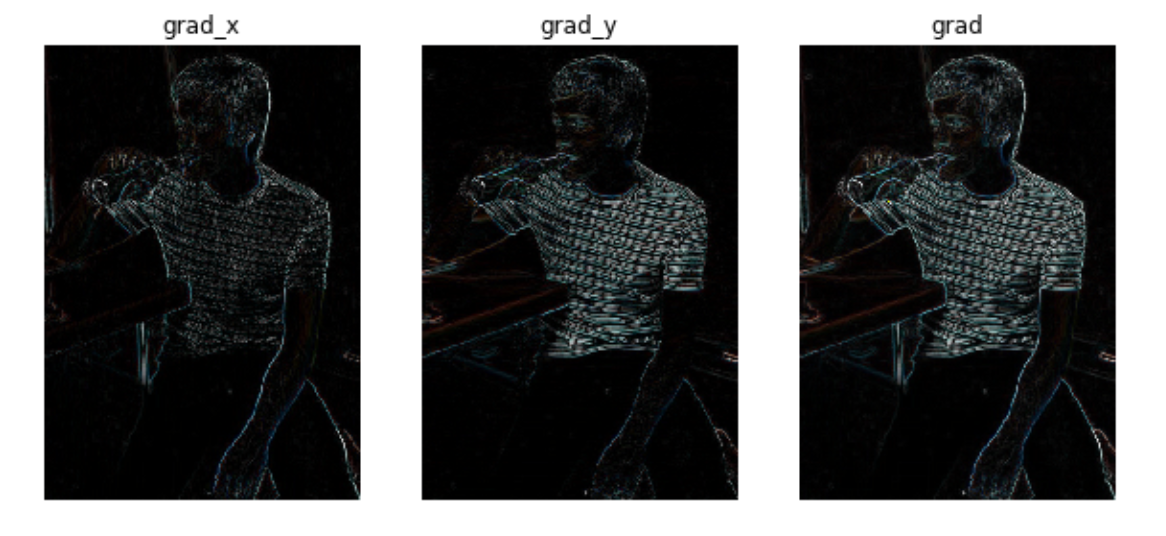
\includegraphics[width=0.9\textwidth]{gradients.png}
  \caption{左:横向梯度绝对值;中:纵向梯度绝对值;右:梯度大小}
  \label{fig:gradients}
\end{figure}

  图\ref{fig:gradients}中包括了RGB三个通道在每一个像素点上的梯度值,在计算HOG特征向量时,我们选取三个通道的梯度的最大值作为该点处的梯度大小,最大值对应的通道的梯度角度为该点处的梯度方向。

  方向梯度直方图统计的实际上是梯度的方向。梯度的方向在$[0^{\circ},360^{\circ})$上,但是我们实际在统计方向时,采用的却是$[0^{\circ},180^{\circ})$的统计范围,计算$\theta(x,y) \mod 180^{\circ}$来代替原有的角度值,即将相差$180^{\circ}$的两个角度视为同一个梯度方向。实验表明,这种统计方式得到的结果往往比采用$[0^{\circ},360^{\circ})$范围的原方向更好\cite{dalal2005histograms}。在统计梯度方向时时,我们还需要使用梯度的大小作为对应方向的权重。

  在计算直方图时,我们取9个组(bins),分别对应$0^{\circ},20^{\circ},40^{\circ},\dots,160^{\circ}$,若一个像素处的梯度正好为20的整数倍,将其梯度大小加到对应的bin中;否则,按照比例,将其加入相邻的两个bins中。以图\ref{fig:distribute}为例。这样一来,HOG特征描述子即为一个长为9的向量,每一个分量的大小对应直方图中相应bin的高度。

\begin{figure}[htb]
  \centering
  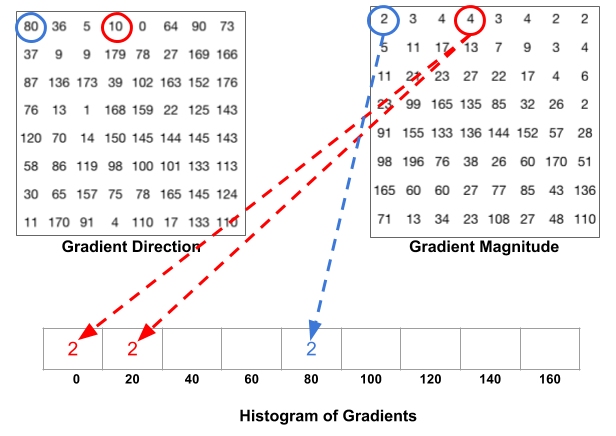
\includegraphics[width=0.7\textwidth]{calc_histogram.png}
  \caption{统计梯度方向直方图的方法示意}
  \label{fig:distribute}
\end{figure}

  值得注意的是,由于图像的梯度是由各像素点周围的颜色值大小计算得到的,所以也会受光照的影响,例如,将所有像素值除以2来使图像变暗,这时所有梯度大小就也会减半,直方图每个bin的高度也会减半。而在一张图片中,每个局部区域的光照可能会有所不同,为了降低这些影响,在进行方向梯度统计时,并不会直接统计一整个图片的方向梯度直方图,而是以$8\times8$像素的区域为一个单元格(cell)来分别进行统计,再在此基础上进行规范化(normalization)。这样会降低光照等噪音对特征描述子质量的影响,使HOG描述子更加稳定鲁棒。此过程如图\ref{fig:procedure}所示。

\begin{figure}[htb]
  \centering
  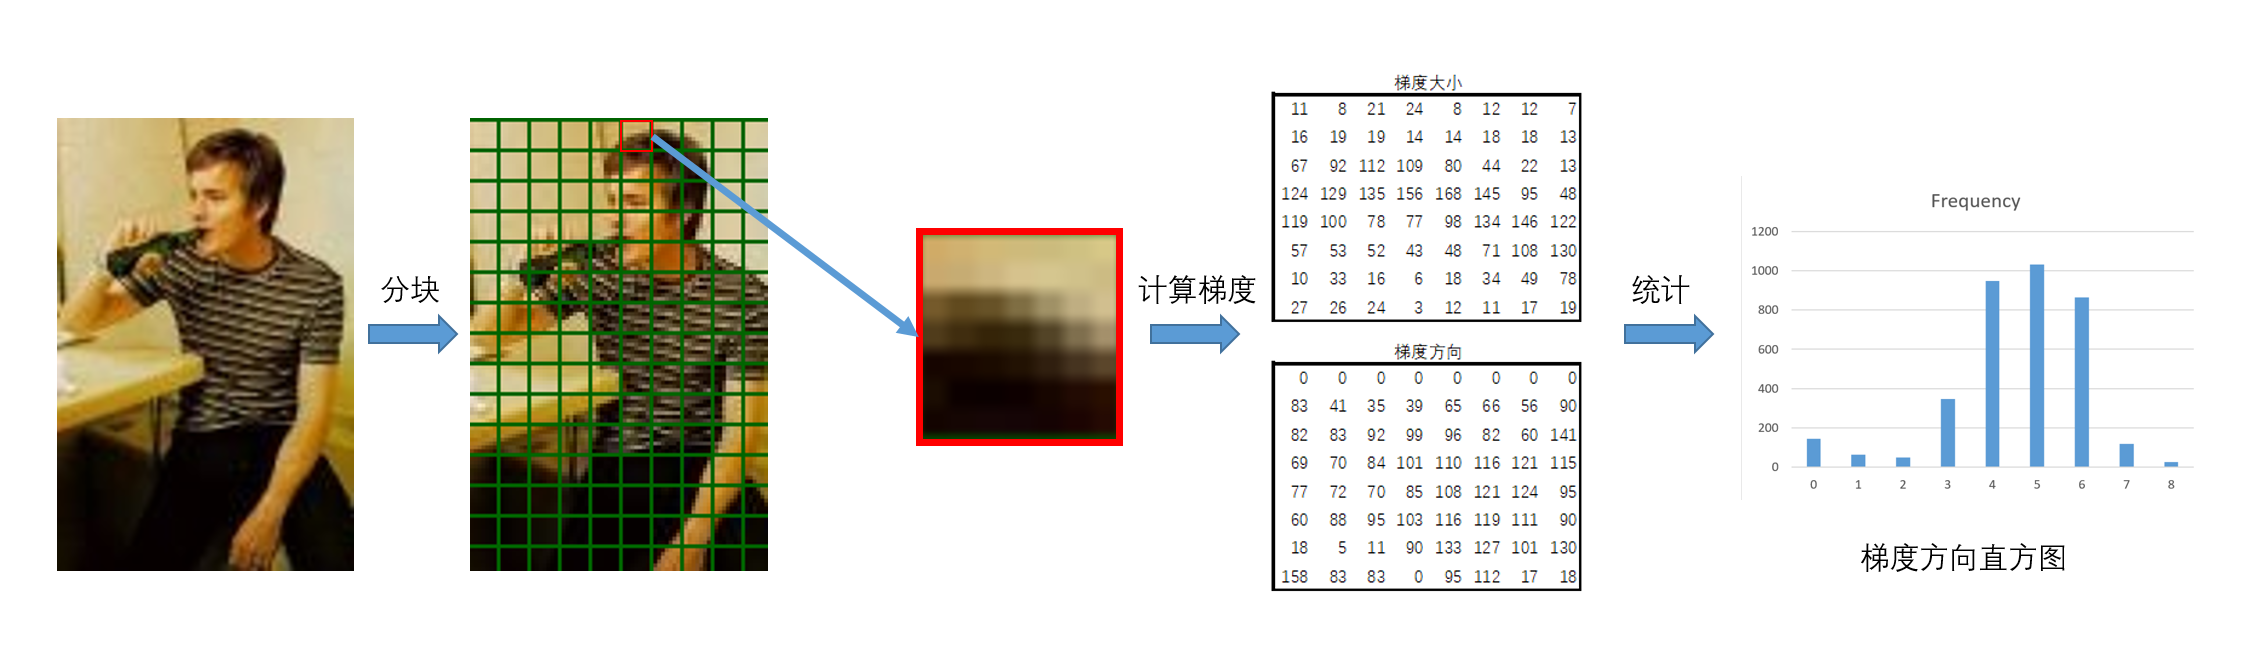
\includegraphics[width=1.1\textwidth]{procedure.png}
  \caption{统计单元格梯度直方图的过程示意图}
  \label{fig:procedure}
\end{figure}

  在进行规范化时,最常用的方法是在单元格的基础上取一个更大的块(block),每块的大小为$16\times16$像素,即包括4个单元格,将每一个块的4个HOG向量作为一个整体进行L2规范化。即$\vec{v}\leftarrow\vec{v}/\sqrt{\lVert v \rVert^2_2 + \epsilon^2}$,其中$\epsilon$为一个足够小的正常数。在规范化一个块之后,我们得到了一个长为36的向量,即这个块最终的HOG向量。再以8像素的步长(stride)移动这个块,对下一个块进行规范化,即两个相邻块之间有2个单元格的重叠。如此循环,直到整张图的每一个单元格都被计算,再将所有经过的块的向量合并在一起,作为整张图的HOG描述子。

\paragraph{尺度不变特征变换}

  尺度不变特征变换(Scale-invariant feature transform,SIFT)是一种不受图片尺度和旋转影响,并在一定程度上不受光照和相机视角影响的特征描述子,它将图像数据转换为有关局部特征的尺度不变坐标。同时,通过在空间和频率域的准确定位,SIFT还可以减少遮挡和噪音带来的干扰。SIFT可以使用有效的算法从图片中提取出大量的独特特征,可以在所有的尺度和位置上密集地覆盖图像,例如,一个$500\times500$像素的图像可以最多生成2000个稳定的特征。SIFT方法中的关键点描述非常独特,可以使单个特征从大型特征数据库中能得到高概率的匹配。但在较为杂乱的图像中,背景中的很多特征可能不会从数据库中得到正确的匹配,故而在正确的匹配之外,生成错误的匹配,不过通过识别关于目标物及其在新图像中的位置,尺度和方向的关键点的子集,可以从完整匹配集中过滤出正确的匹配\cite{lowe2004distinctive}。

  为了最大限度地降低提取特征的成本,使用级联过滤(cascade filtering)方法来检测关键点,先使用高效的算法来检测出一些侯选位置,然后再进一步详细检查,将更加耗时的计算只运用到通过了初始测试的候选点位置。

  \citet{lowe2004distinctive}提出的SIFT生成图像特征的主要步骤如下:

  I. 尺度空间极值检测:通过高斯差分方程(difference-of-Gaussian function),在所有可能的尺度下搜索稳定的特征,来找出尺度和方向不变的潜在相关点。对于输入图像$I(x,y)$和可变尺度高斯核函数$G(x,y,\sigma)$,可以计算出图像的尺度空间$L(x,y,\sigma)$:
$$L(x,y,\sigma)=G(x,y,\sigma)\ast I(x,y)$$

  “$\ast$”为$x,y$上的卷积计算操作,$G(x,y,\sigma)=\frac{1}{2\pi\sigma^2}e^{-(x^2+y^2)/2\sigma^2}$,$\sigma$为尺度空间因子,反映了图像被模糊的程度,$\sigma$越大,对应的尺度也越大。

  为了有效地检测出尺度空间中稳定的关键点位置,使用高斯差分方程来与图像进行卷积,由一个常数因子$k$,得出$D(x,y,\sigma)$:
$$D(x,y,\sigma)=(G(x,y,k\sigma)-G(x,y,\sigma))\ast I(x,y)=L(x,y,k\sigma)-L(x,y,\sigma)$$

  为了检测中$D(x,y,\sigma)$函数的局部最大值和最小值,每个点都与它在同尺度上的8个邻点,以及相邻的两个尺度上的各9个邻点相比较(相邻尺度上$\sigma_{s+1}=k\dot\sigma_s$)。只有它的值比相比较的26个相邻点都要小或者都要大时,才选取该点作为候选点。

  II. 关键点精确定位:对每个候选点上,拟合一个精细的模型来确定其位置和尺度,并根据其稳定性来选择关键点。

  对尺度空间函数$D(x,y,\sigma)$进行最多二阶的泰勒展开:
$$D(\vec{x})=D+\frac{\partial D^T}{\partial \vec{x}}\vec{x}+\frac{1}{2}\vec{x}^T\frac{\partial^2D}{\partial\vec{x}^2}\vec{x}$$

  其中$D$和其微分在给定候选点处被计算,$\vec{x}=(x,y,\sigma)^T$是相对于该点的偏移向量。为了求$D$的局部极值的位置,对上式求导并设$D'$为0,则极值的位置的偏移量$\hat{\vec{x}}$和$D$的局部极值点分别为:
\begin{gather*}
\hat{\vec{x}}=-\frac{\partial^2 D^{-1}}{\partial \vec{x}^2}\frac{\partial D}{\partial \vec{x}}\\
D(\hat{\vec{x}})=D+\frac{1}{2} \frac{\partial D^T}{\partial \vec{x}} \hat{\vec{x}}
\end{gather*}

  为了保证极值点的稳定性,需要剔除低对比度的极值点。若$|D(\hat{\vec{x}})|$的值小于0.03(假定每个像素的值的大小在$[0,1]$之间),则将该极值点舍弃。

  III. 方向赋值:根据局部的图像梯度方向,将一个或多个方向赋值给每个关键点位置。后续在该图像上进行的所有操作都将根据为每个特征所指定的方向、尺度和位置进行变换(transform),从而为这些特征提供方向、尺度不变性。

  得到了每个关键点的尺度$\sigma$后,由特征点为中心,计算出同一尺度下周围区域每个点$(x,y)$的梯度大小$m(x,y)$和方向$\theta(x,y)$:
\begin{gather*}
m(x,y)=\sqrt{(L(x+1,y)-L(x-1,y))^2+(L(x,y+1)-L(x,y-1))^2}\\
\theta(x,y)=\tan^{-1}((L(x,y+1)-L(x,y-1))/(L(x+1,y)-L(x-1,y)))
\end{gather*}

  使用直方图统计关键点邻域内像素对应的梯度方向和大小。

  IV. 生成特征描述子:校正旋转门主方向以确保旋转不变性,生成关键点描述子并进行归一化处理,以去除光照的影响。

  SIFT准确率较高,对于尺度和旋转不敏感,但由于求SIFT特征向量计算量较大,耗时较长,所以在需要实时图像识别时并不常被使用。

\subsubsection{分类器}

  分类器的作用是将图像的矩形区域分类为目标对象或背景。分类器的训练需要正负样本,分别对应目标区域和背景区域。在对分类器进行一定规模的训练后,此时将一个图像上的区域块的特征向量作为分类器的输入,分类器即会输出该区域包含目标物体的概率。

  在实际使用时,得到了一个图像帧后,选取不同的尺度,尺度决定了检测窗口的大小,然后在图像上选取相应尺度的检测窗口,计算它的特征向量,使用分类器得出其中包含目标物的概率,如果这个概率超过给定的阈值,则认为该检测窗口中即包括待追踪物体。在检测完一个追踪窗口后,按照给定的步长在图像上滑动检测窗口,继续进行检测,直到整个图片在所有给定尺度上都被检测过。

\paragraph{SVM}

// TODO

\paragraph{AdaBoost}

// TODO


\subsection{基于动态的追踪}

  在基于动态的追踪中,我们假定在此前的几乎所有帧中都已成功地跟踪了对象,并保有对其运动模式和之前位置的记录,目标是根据这些已有信息找到在当前帧中物体的位置。物体的运动模型给了一个它当前位置的粗略预测,此外,还需要根据该目标对象在先前的帧中的外观记录(即特征)对物体的位置进行更加精确的估计,我们仍可以使用在目标检测中提过的物体特征,如颜色直方图,HOG等。根据这些外观的模型和特征,我们可以在由物体运动模型所预测的物体位置的邻域中进行搜索,以提高速度和准确度。根据外观进行分类的原理与目标检测相同,但如何将物体的运动模型等信息目标检测结合起来,就需要使用下面提到的几种算法。

\subsubsection{Boosting算法}
  在目标追踪中,我们常使用在线分类器进行目标识别,即在运行时即使训练的分类器。分类器的训练过程中,最初的正样本由使用者提供,在一张包含目标人物的图像中手动或使用某种检测算法选出一个框(bounding box,bbox)。分类器将该图像中的bbox作为正样本,在bbox之外取出若干个负样本进行训练拟合。

  在收到下一帧后,在物体原位置的所有相邻的位置上运行分类器,取得分最高的一个bbox作为当前帧的物体位置,再以当前帧检测出的bbox作为正样本,背景中提取负样本继续训练分类器。Boosting算法原理非常简单,相应地,追踪效果也比较平庸,由于它每次会选择得分最高的位置作为当前帧的检测结果,可能并不能选取到正确的目标位置,且容易出现漂移现象。

  在Boosting算法的基础上,\citet{babenko2009visual}提出了多示例学习(multiple instance learning,MIL)算法。不同于传统的分类器将每一个实例进行分类的方法,MIL将若干个实例归到一个包(bag)中,即正样本包和负样本包。只要包中的一个图像是正样本,就将其认为是正样本包,相对的,只有包中所有实例均为负样本,才将其认为是负样本包。构建正样本包的方法是首先包含目标物在当前图像中的图像块,并以此为中心,将该位置周围的小邻域中的图像块都包括其中。这样以来,即使被跟踪对象的当前位置不准确,只要将目标物作为中心的图像块被作为邻域放入了正样本包中,分类器就可以以它进行训练。

  但Boosting和MIL算法都有着共同的缺点,它们难以判断出是否已经对目标物失去了追踪而错误地选定了其他位置,此外,当目标物在一段时间内被遮挡的情况下,它们都难以恢复追踪。

\subsubsection{卡尔曼滤波}

  卡尔曼滤波是一种假定目标物体的运动服从线性高斯分布,以此对目标的运动状态进行预测,将预测结果与观察模型进行比较,根据误差更新预测模型,估计物体的当前位置的方法。它不是单纯地在前一帧目标物位置周围作检测,而是主动对其运动状态进行建模,预测它即将出现的位置。
  
  卡尔曼滤波器是一组提供最小二乘法的有效递归解的数学方程,它可以对于系统的过去、当前、甚至未来状态的进行估计\cite{welch1995introduction}。

  卡尔曼滤波器对离散时间的控制过程的状态$x\in \real^n$进行估计,该过程可以由一个马尔科夫链表示:
$$x_{k+1}=\mat{A}_k x_k + \mat{B} u_k + w_k$$

  同时,提供了对系统当前状态的测量$z\in \real^m$:
$$z_k=\mat{H}_k x_k + v_k$$

  其中,随机变量$w_k$和$v_k$分别表示系统和测量误差,假定它们是互相独立的,并服从正态分布:
\begin{gather*}
p(w)\sim N(0,Q),\\
p(v)\sim N(0,R).
\end{gather*}
  
  $n\times n$的矩阵$\mat{A}$将系统在时间$k$和$k+1$时的状态相关联起来,不存在驱动函数或系统噪音。$n\times l$的矩阵$\mat{B}$将控制输入$u\in \real^l$与系统状态$x$相关联。$m\times n$的矩阵$\mat{H}$将系统状态和对系统的测量$z_k$相关联。

  我们根据时间$k$前的过程,计算$\hat{x}^{-}_k \in \real^n$作为为时间$k$时的先验(a priori)状态估计,并根据对系统状态的测量$z_k$计算后验(a posteriori)状态估计$\hat{x}_k \in \real^n$。我们将先验和后验估计误差定义为:
$$e^{-}_k \equiv x_k -\hat{x}^{-}_k, e_k \equiv x_k - \hat{x}_k. $$

  则先验和后验估计误差协方差分别为:
\begin{gather*}
P^{-}_k = E[e^{-}_k {e^{-}_k}^T],\\
P_k=E[e_k {e_k}^T]
\end{gather*}

  使用先验估计$\hat{x}^{-}_k$和实际测量$z_k$来计算后验状态估计$\hat{x}_k$:
$$\hat{x}_k = \hat{x}^{-}_k + \mat{K} (z_k - \mat{H}_k \hat{x}^{-}_k)$$

  在上式中,$\mat{H}_k \hat{x}^{-}_k$是根据先验估计对测量值的预测,$(z_k - \mat{H}_k \hat{x}^{-}_k)$被称为测量残差(residual)。残差反映了先验估计及预测方法相对于实际测量的插值。$n\times m$的矩阵$\mat{K}$是最小化后验误差协方差的增益(gain)。将上式代入求$P_k$的公式中,取结果相对于$\mat{K}$的导数,并设为0,可以求得:
$$\mat{K}=\frac{P^{-}_k \mat{H}^T_k}{\mat{H}_k P^{-}_k \mat{H}^T_k + \mat{R}_k}$$

  由上式可以得出,$R_k$为了测量误差协方差,当它趋于0时,$\mat{K}$越大,特别地:
$$\lim_{R_k \to 0} \mat{K}_k=\mat{H}^{-1}_k$$

  另外,当先验估计误差协方差$P^{-}_k$趋于0时,$\mat{K}$越小,特别地:
$$\lim_{P^{-}_k \to 0} \mat{K}_k=0$$

  所以,当测量误差协方差$R_k$约接近0时,实际测量$z_k$更加被取信,而预测的测量值$\mat{H}_k \hat{x}^{-}_k$更不被相信,而当先验估计误差协方差$P^{-}_k$趋近于0时则相反。
  
  现在我们就有了根据先验估计和测量计算后验状态估计的方法。后验状态估计反映了状态分布的数学期望,根据$w,v$的分布,状态概率分布也应当满足正态分布,而后验估计误差协方差则反映了状态分布的误差。故:
$$p(x_k|z_k)\sim N(E[x_k],E[(x_k-\hat{x}_k)(x_k-\hat{x}_k)^T])=N(\hat{x}_k,P_k)$$

  卡尔曼滤波分为两组方程:时间更新方程和测量更新方程。时间更新方程根据当前状态和误差协方差估计,预测下一时间的先验估计;测量更新方程用于根据所获得的新的测量,再结合先验估计来获取一个已优化的后验估计,这个后验估计又被传回时间更新方程。如此循环,完成一个预测-矫正的过程,以自动化地对模型进行更新,对状态进行估计。

  时间更新方程包括:
\begin{gather*}
\hat{x}^{-}_{k+1}=A_k \hat{x}_k + B u_k \\
P^{-}_{k+1}=A_k P_k A^T_k + Q_k
\end{gather*}

  测量更新方程包括:
\begin{gather*}
K_k=P^{-}_k H^T_k(H_k P^{-}_k H^T_k + R_k)^{-1} \\
\hat{x}_k = \hat{x}^{-}_k + K (z_k - H_k \hat{x}^{-}_k) \\
P_k = (I-K_k H_k)P^{-}_k
\end{gather*}

  $Q_k$和$R_k$均为常数,分别与$w$和$v$相关,估计误差协方差$P_k$和增益矩阵$K_k$将会在计算中迅速收敛,并保持不变。

  卡尔曼滤波器限定了系统噪声必须符合正态分布,且必须为线性系统,而在实际使用中,很难同时满足要求,此时精度就会较低。

\subsubsection{粒子滤波}

  粒子滤波器(particle filters)是一种基于概率密度的粒子表示的顺序蒙特卡洛方法(sequential Monte Carlo methods),它可以应用在任意状态-空间模型,可以对非线性、非高斯系统的动态进行建模,是传统的卡尔曼滤波的一般化方法\cite{arulampalam2002tutorial}。

  首先对跟踪目标进行建模,并定义一种相似度度量确定粒子与目标的匹配程度。在目标搜索的过程中,它会先按照一定的分布(比如均匀分布或高斯分布)在全局撒一些粒子,统计这些粒子与目标的相似度,确定目标可能的位置。在可能性较高的位置上,下一帧加入更多新的粒子,确保在更大概率上跟踪上目标。

  首先随机散布一些粒子$\{x^i_{0:k},i=0,\dots,N_s\}$,它们分别具有权重$\{w^i_k,i=1,\dots,N_s\}$,其中$x_{0:k}=\{x_j,j=0,\dots,k\}$是时间0到$k$间所有状态的集合。则时刻$k$时,后验概率密度可被估计为:
$$p(x_{0:k}|z_{1:k})\approx \sum^{N_s}_{i=1} $$

  粒子滤波器相对于卡尔曼滤波器,虽然适用范围更广,但计算量也更大

\subsubsection{MeanShift和CamShift}

These are algorithms for locating the maxima of a density function. They are also used for tracking.

\subsubsection{相关滤波}

  相关滤波算法利用了在傅里叶域中,两个矩阵的卷积可以被转换为逐元素的点乘的性质,在达到与以往的更加复杂的算法的效果的基础上,降低了计算所需要的资源和时间。在相关滤波中,目前效果最佳,也最常用的是KCF算法(Kernelized Correlation Filters),由\citet{henriques2015high}在2015年提出。

  KCF算法中有三种核函数,包括线性核函数、多项式核函数和高斯核函数。首先使用线性核函数为例,在线性回归函数中使用岭回归(Ridge Regression)以得到一个简单的闭式解。通过训练得到一个函数$f(\vec{z})=\vec{w}^T\vec{z}$,使得样本$\vec{x}_i$及其回归目标$y_i$之间的方差最小,即:
$$\min_{\vec{w}}\sum_i (f(\vec{x_i})-y_i)^2+\lambda \lVert\vec{w}\rVert^2$$

  类似SVM,这里的$\lambda$是用于防止过拟合的正则化参数。由于岭回归的性质,上式可以得到一个简单的闭式解$\vec{w}=(X^TX+\lambda I)^{-1}X^T\vec{y}$。其中矩阵$X$的第$i$行为$\vec{x}_i$,向量$\vec{y}$的第$i$个元素为其回归目标$y_i$。$I$为单位矩阵。上面已经提过,为了提高运算效率,将计算转到傅里叶域中进行,故数据一般都以复数计算,所以将矩阵装置替换为共轭转置,得到:
$$\vec{w}=(X^HX+\lambda I)^{-1}X^H\vec{y}$$

  这个公式已经可以进行对$\vec{w}$的计算了,但是由于计算中包括矩阵求逆,计算量很大,难以符合实时性要求。\citet{henriques2015high}巧妙地利用了循环矩阵的性质和离散傅里叶变换,将该运算简化成只需要元素点乘的版本,大大提高了运行速度。具体推导如下:

  以单通道一维信号输入为例,对于一个$n\times1$的向量$\vec{x}$,以它为生成向量计算一个循环矩阵$X$:

$$
X = C(\vec{x}) =
\left[
\begin{matrix}
 x_1      & x_2      & x_3      & \cdots & x_n     \\
 x_n      & x_3      & x_2      & \cdots & x_{n-1} \\
 x_{n-1}  & x_n      & x_1      & \cdots & x_{n-2} \\
 \vdots   & \vdots   & \ddots   & \ddots & \vdots  \\
 x_2      & x_3      & x_4      & \cdots & x_1     \\
\end{matrix}
\right]
$$

  循环矩阵的模式是确定的,并完全由它的生成向量向量$\vec{x}$决定。该矩阵的每一行都是$\vec{x}$的一种循环位移向量。可以相当于将正样本图像向上/下移动不同的像素来得到新的样本,类似于MIL分类器中在正样本周围邻域取正样本包的做法,相当于增加了样本的数量,使分类器的效果更好。

  特别的是,循环矩阵有一个重要的特性,即对任意生成向量$\vec{x}$,所有循环矩阵都可被离散傅里叶变换(DFT)对角化,即:
$$X = F {\rm diag}(\hat{\vec{x}}) F^H$$

  其中$\hat{\vec{x}}$为$\vec{x}$的离散傅里叶变换,$F$为一个与$\vec{x}$无关的常数矩阵,称为离散傅里叶变换矩阵(DFT matrix),它可以用于计算所有向量的离散傅里叶变换,即$\mathcal{F}(\hat{z})=\sqrt{n}F\vec{z}$。由此,如果我们将输入数据都用其循环矩阵表示,则可以得到:
$$X^HX = F {\rm diag}(\hat{\vec{x}}^\ast)F^H F {\rm diag}(\hat{\vec{x}})F^H$$

  其中$\hat{\vec{x}}^\ast$为$\hat{\vec{x}}$的复共轭向量,由于对角矩阵是对称的,所以共轭转置的结果即为原矩阵的复共轭。此外,根据$F$的性质,$F^H F $即为单位矩阵$I$。此外,由于在对角矩阵上进行的运算是逐元素的,我们使用$\odot$表示向量或矩阵间的逐元素点乘,则上式可以简化为:
$$X^HX = F {\rm diag}(\hat{\vec{x}}^\ast \odot \hat{\vec{x}}) F^H$$

  将这个公式带入求$\vec{w}$的公式中,可以最终将$\vec{w}$的计算过程简化成:
$$\hat{\vec{w}}=\frac{\hat{\vec{x}}^\ast \odot \hat{\vec{y}}}{\hat{\vec{x}}^\ast \odot \hat{\vec{x}}+\lambda}$$

  这里的分数代表逐元素的除法。在求出$\hat{\vec{w}}$后,可以通过很简单的元素求出其的逆离散傅里叶变换。

  //除了线性回归之外,还可以使用核函数拟合出非线性回归。在KFC方法中,非线性回归效率在训练和评估时都可以做到和线性回归相似的效率。首先设函数$\varphi(\vec{x})$用于将线性输入特征向量映射到非线性空间。

// TODO

  KCF算法是缺点是对尺度变化的适应性不强。

\subsubsection{MedianFlow}
  MedianFlow算法从时间向前和向后的两个方向来追踪物体,并测量这两个轨迹之间的差异。最小化这个向前/向后差异,既可以稳定可靠地检测跟踪失败,以及选择视频中的可靠轨迹。

\subsubsection{GOTURN}

  GOTURN是一个基于卷积神经网络(convolutional neural networks,CNN)的跟踪算法,它对于视角的变化、光照、变形等具有鲁棒性,但不能很好地处理遮挡。

\subsubsection{CSR-DCF算法}
  通道和空间稳定的判别性相关滤波器(Discriminative correlation filter with channel and spatial reliability,CSR-DCF)由\citet{lukezic2017discriminative}在2017年提出,根据实验,它有着比KCF算法更高的精度,相对的,帧率较KCF更低。

\subsubsection{深度学习}

\section{激光行人追踪}
激光行人追踪的方法主要是对人双腿的追踪。在激光图像中,人的双腿在有一种明显的模式,即max-min-max-min-max。

% !TeX root = ../main.tex

\chapter{ROS导航和可佳导航简介}

\section{ROS导航}

ROS(Robot Operating System)是一个开源的专用于机器人软件开发的操作系统。ROS中提供了一个模块化的简单2D导航系统ROS Navigation,其主要架构如图\ref{fig:rosnav}所示。

\begin{figure}[htb]
  \centering
  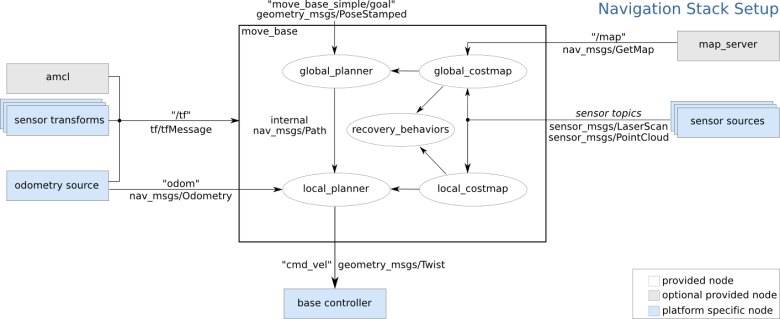
\includegraphics[width=1.1\textwidth]{ROS_navigation_stack.png}
  \caption{ROS导航架构}
  \label{fig:rosnav}
\end{figure}

\subsection{建图}
  包括gmapping\cite{grisetti2007improved}和cartographer\cite{hess2016real}两种方法。

\subsection{定位}
  amcl是有图后的定位模块,使用粒子滤波算法进行对机器人当前位置的估计。

\subsection{costmap}

  地图表示与更新。

\subsection{导航控制}

  导航控制模块即图\ref{fig:rosnav}中的move base模块。包括全局规划器、局部规划器和恢复机制。

\section{可佳导航}

\begin{figure}[htb]
  \centering
  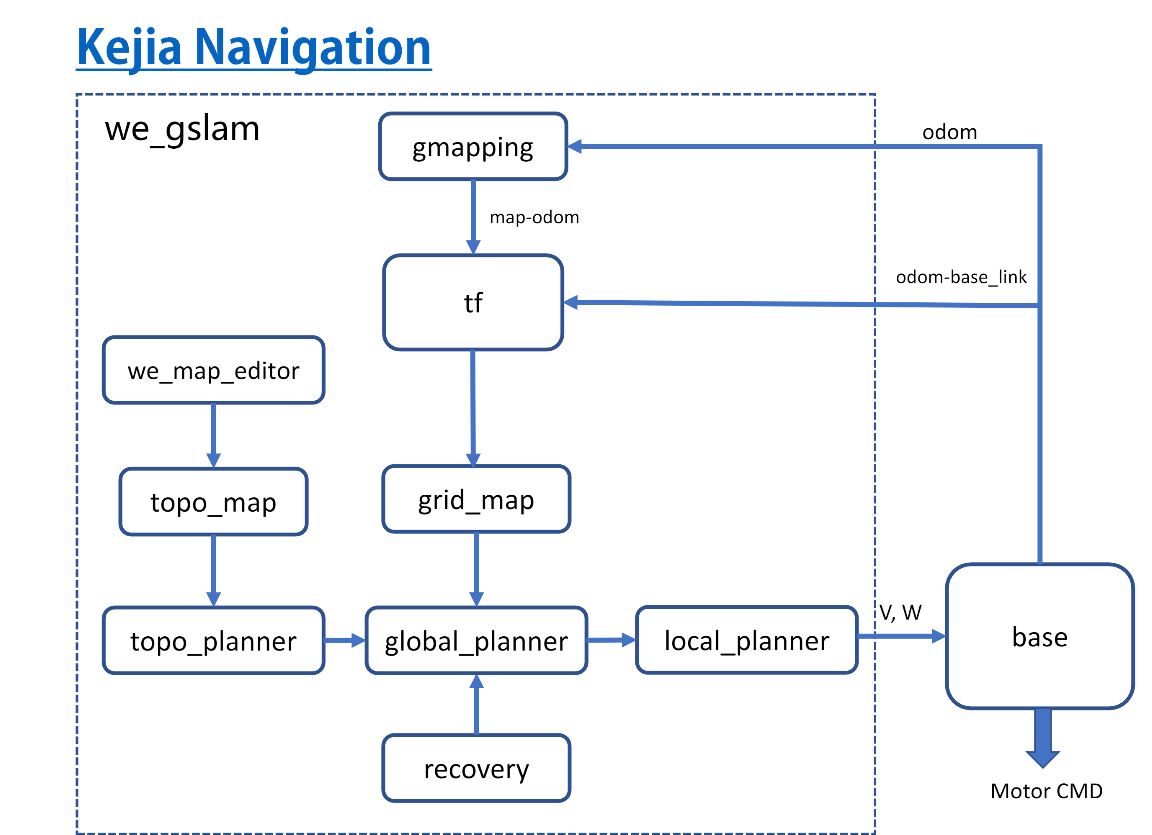
\includegraphics[width=1.1\textwidth]{kejianav.png}
  \caption{可佳导航架构}
  \label{fig:kejianav}
\end{figure}

  可佳导航的架构如图\ref{fig:kejianav}所示。在导航方面,它相对于ROS导航,还加入了拓扑导航。使用VFH(vector field histogram)\cite{borenstein1991vector}进行局部避障。
% !TeX root = ../main.tex

\chapter{以可佳机器人为基础的行人追踪系统}

\section{输入设备}

\subsection{Kinect}

  Kinect深度相机可以同时为机器人提供RGB图像和深度图像的输入,经过对齐后,便可以简单地通过目标在RGB图像上的位置得到目标相对于机器人的坐标。

  但Kinect的深度图像也有一定的不足。使用RGB-D相机Kinect作为彩色图像和深度信息的输入,而Kinect的深度图像只能有效判断80厘米之外的物体的距离,且由于Kinect通过红外发射器和红外摄像头来获得深度信息,所以受阳光照射的影响较大,所以在实际使用中,Kinect深度图像可能会出现不稳定和空洞现象。对于Kinect的深度图像在近距离精度较低的现象,可以考虑在较近距离内使用2D激光进行行人的3D位置判别。对于Kinect的空洞现象,考虑使用KinectFusion算法\cite{newcombe2011kinectfusion}或OctoMap\cite{hornung2013octomap},将深度图像投影到RGB图像中,以进行对相机视野中场景的3D重建。

\subsection{2D激光}

  由于本文中的行人检测与追踪算法主要使用了视觉信息,所以这里2D激光主要用于建图、定位和导航。定位和导航在本文中不是主要内容,所以不再特别赘述。

\section{视觉追踪系统}

  视觉追踪系统是行人跟随系统最为核心的模块。在第三章中已经对ROS导航和可佳导航进行了调研,二者都有较为稳定鲁棒的导航功能。在通过视觉追踪系统得到行人在RGB图像中的位置后,通过对齐Kinect中的深度图像便可以得到行人在地图中的3D位置。将该位置设置为导航系统的目标,并调用ROS导航或可佳导航的导航模块,同时保持机器人和行人保持一定的距离,便可以实现稳定的行人跟随系统。

\subsection{总体架构}

\subsubsection{目标人物注册}

  追踪系统在初始化时需要得到目标行人所在的大致位置,即提供行人在初始帧中的界限框(bounding box),并由此对追踪器和分类器进行初始化。为了能够有效地对目标用户进行识别,这里采用开源系统OpenPose\cite{cao2018openpose}来进行人体的骨骼识别。OpenPose系统不仅可以判断出图像中所有人物的骨骼信息,还可以对人物的姿势进行识别,这带来了另一个好处,即我们可以要求被跟随的目标站在机器人前方做出一个指定的姿势,如举起右手,直到机器人提示注册成功,这样一来,我们就可以在对目标人物的特征没有先验知识的情况下在初始化时发现目标了。

\subsubsection{行人追踪器}
  根据VOT2017的结果\cite{kristan2017visual},CSR-DCF算法在实时实验中取得了最佳的结果,由于其出色的性能和实时性的良好实现,选用CSR-DCF作为追踪器。CSR-DCF追踪器是一种相关滤波追踪器,它将HOG和颜色特征相结合,并提出了空间和通道置信度来对追踪器进行调整。在实际测试中,CSR-DCF算法可以达到约40FPS的帧率,达到实时性要求。相对于其他速度更快的算法,如MedianFlow、MOSSE、CamShift算法,CSR-DCF算法更为准确,在一定程度上对于遮挡鲁棒。帧率相对较高的KCF追踪器在尺度不变的情况下也能做到相似的准确程度,能在一定程度上解决目标被遮挡的问题,且有可能在失败后再次恢复,但前面已经讨论过,KCF算法无法适应目标尺度大小的变化。另一个适应于长期追踪的TLD算法,识别准确率较低,边界框会经常跳动或漂移,甚至会经常检测到错误的位置,但在目标在视野中消失一段时间后再回到画面时,TLD算法能识别到目标的回归并继续对其追踪。

  在实际使用时,CSR-DCF算法最大的缺点即为它几乎无法从跟踪失败中恢复,且对于错误的情况,CSR-DCF算法常常不能及时发现。既然选用了CSR-DCF算法,并想使用它来完成一个长期追踪的任务,这就成为了必须克服的问题。为此,在系统中加入一个分类器,该分类器在追踪时检测追踪器是否发生错误,并在追踪器追踪失败时尝试找回目标、帮助重新建立追踪。

\subsubsection{分类器}
\paragraph{分类器的选择}
  分类器通常要结合人工特征来使用,在行人识别中,最为常用的特征即为HOG特征。HOG特征和SVM分类器的组合从\citet{dalal2005histograms}最先提出开始,就在行人检测领域取得了重大的成果和最好的效果。但由于HOG检测的是人体的轮廓特征,对于形变和快速运动效果不好,当图像分辨率较低时效果也会变差。此外,HOG对于不同行人之间进行分辨效果也不佳。由于HOG特征的这些缺点,同时引入颜色直方图来对图像信息做补充。颜色直方图对光照变化和背景颜色相似的情况较为敏感,对目标的细节信息和颜色的相对位置不关注,但这些问题可以由HOG来代为弥补,而颜色直方图没有边界效应,对快速运动不敏感,且由于不同行人的衣着不同,对于不同行人的分辨也起到很大作用。所以在本文中使用HOG特征和HSV直方图中的H、S直方图结合起来描述目标的特征。

  为了分类精度,使用高斯核的SVM分类器进行分类。为了减少运行时计算量,且避免错误的追踪结果污染分类器的情况,这里仅仅对分类器进行一次初始化而不是采用在线学习的机制。

\paragraph{分类器的初始化}

  在训练分类器时,需要正负样本,负样本从图像背景中提取,正样本即为目前目标所在图像区域。为了增加样本的数量,提高分类器准确度,采用以下两个方法:
  
  a. 在建立起追踪后,提取一定数量的帧后再进行训练。如设定提取前100帧的图像,这个过程约为5秒时间,在这段时间内,假设追踪器不会出现错误且目标不会被遮挡;但如果在这段时间内,由于物体离开视野或严重变形等原因导致追踪器发生失败,则立即将收集到的正负样本传给分类器进行学习。

  b. 参考类似MIL追踪器的思想,通过将初始帧进行一定的旋转、位移、尺度变化等操作增加正样本数量。如随机将物体所在界限框平移不超过$10\%$的距离,旋转不超过$5^{circ}$的角度,进行$5\%$以内的缩小或放大,取新的界限框在图像中的区域,或对原图像进行镜面翻转、高斯模糊等操作,将这些得到的新图像块加入正样本,便可以大大提高正样本的数目。取负样本时,通过在界限框之外随机取背景图像即可达到需要的数目。

\paragraph{检测和恢复追踪器的错误}
  由于运行分类器的速度要明显慢于运行追踪器的速度,并不会对每一帧追踪器的结果进行验证,而是每10帧左右将当前追踪器得到的图像块输入到分类器中得到一个分数,即它属于正样本的概率。设置一个阈值$fail\_thred$,当得分小于该阈值时,认为当前图像块非目标区域。但是在追踪任务中,经常会出现目标发生形变和被遮挡的情况,追踪器可以对这些情况在一定程度上鲁棒,但分类器就会对其此时的结果直接否定。针对这种情况,设置一个能容忍分类器报错的最大次数,当分类器连续报错超过此阈值时,认为追踪器出错,误追踪了其他对象,否则认为是目标短暂地发生了形变或受到了遮挡,不对追踪器进行更新。

  当判断追踪器发生错误或追踪器自身发生失败时,使用分类器对当前帧进行不同尺度上的全局扫描,进行目标行人的搜索。在这个过程中,记录全局扫描中得到的得分最高的图像块,若其得分超过一个阈值$positive\_thred$,则认为该图像块包含目标,否则确认目标丢失。


\begin{figure}[htb]
  \centering
  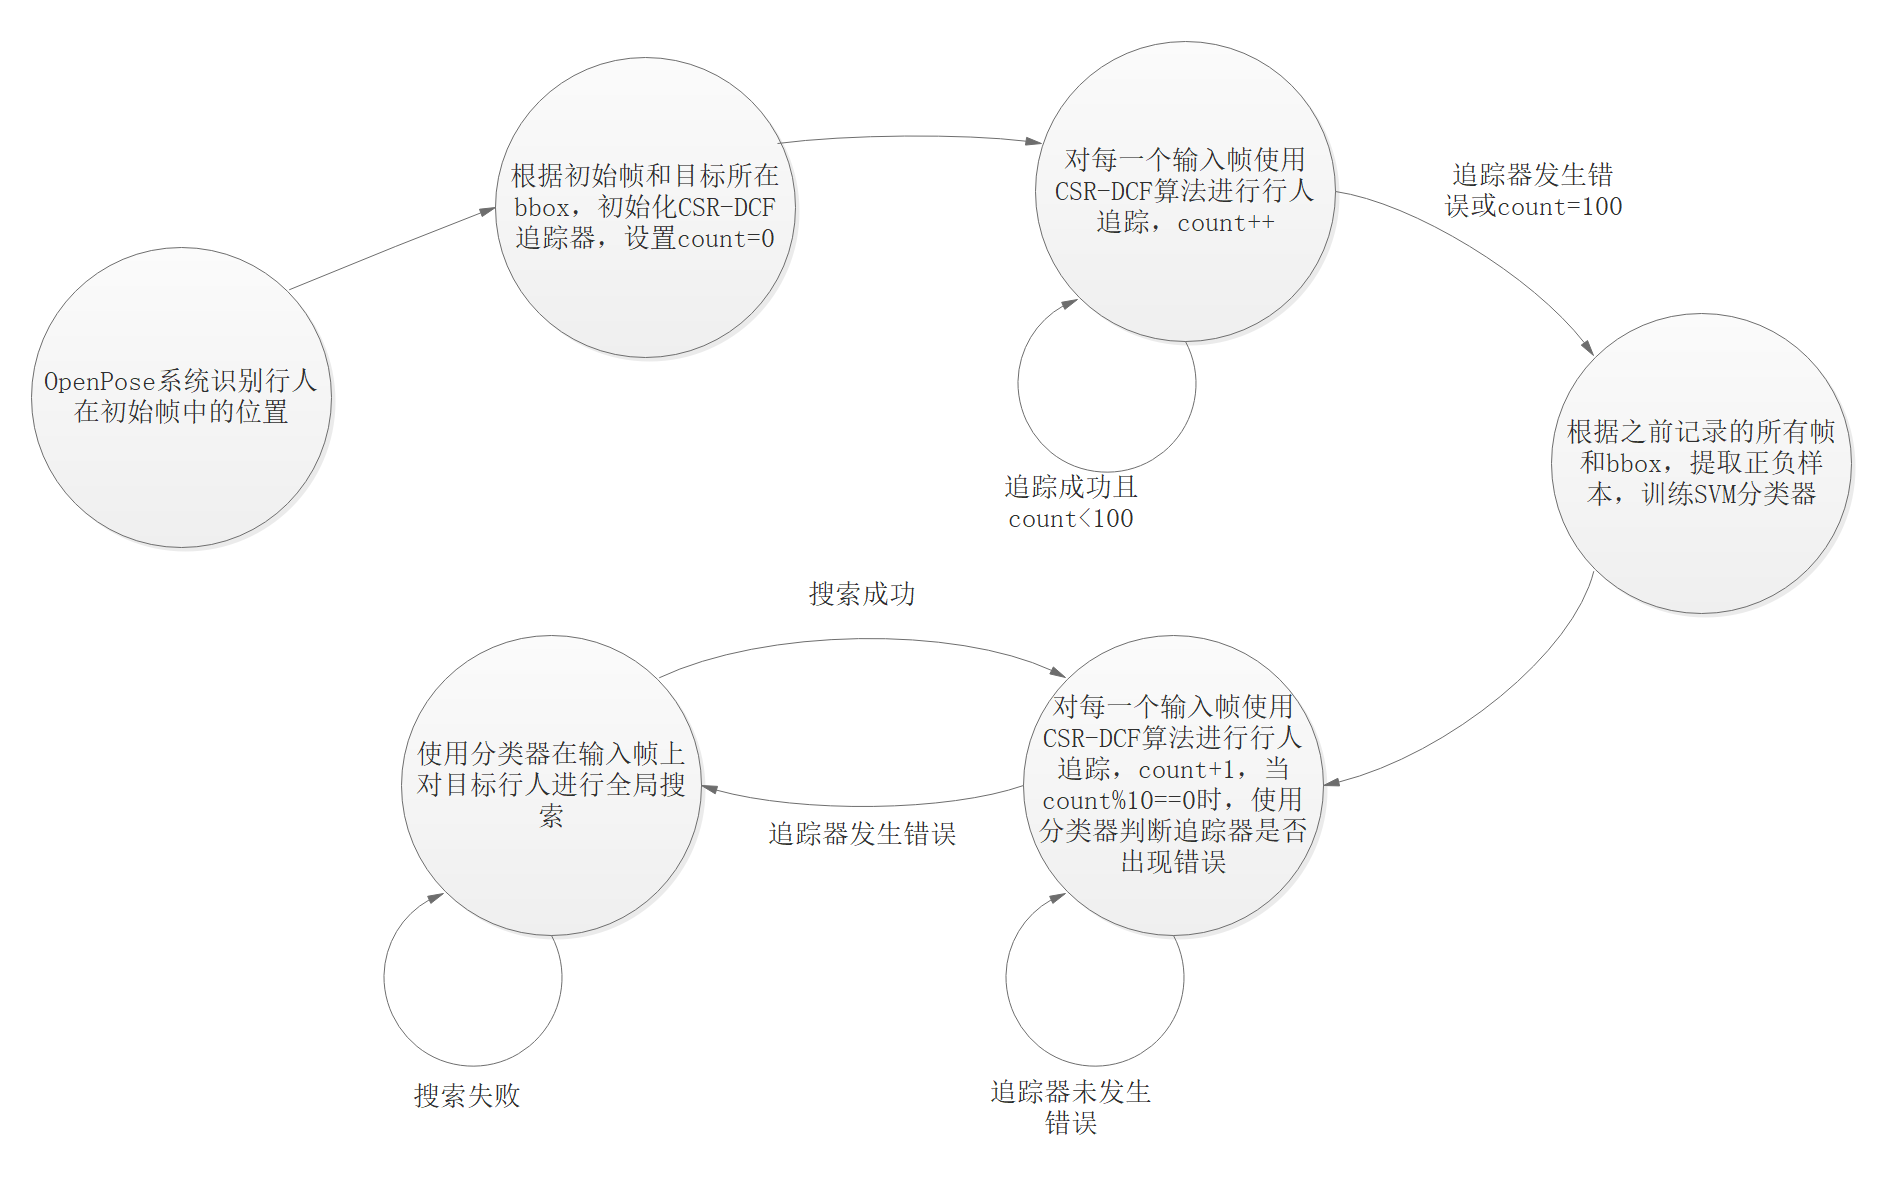
\includegraphics[width=1.1\textwidth]{statemachine.png}
  \caption{有限状态机}
  \label{fig:statemachine}
\end{figure}

\subsubsection{目标丢失恢复}

  当追踪失败且分类器也未能发现物体时,认为目标丢失,此时有几种可能:(1)目标从视野的左右两侧消失;(2)目标被完全部分或完全遮挡,如进入了另外的房间;(3)目标发生严重形变,或因光照的变化导致分类器检测失败。

  对于情况(1)和(2),相对于静态相机进行追踪时只能等待行人回到视野,机器人上的行人追踪系统可以使机器人主动转动视角或前往行人上一个出现的位置,来及时地恢复对行人的追踪。

  由于CSR-DCF追踪器几乎不能处理目标丢失后的恢复工作,使用分类器以一定频率对于输入帧进行全局扫描,当重新检测到目标时,重新初始化追踪器,建立追踪。


\subsubsection{总体结构}
  把初始化过程、追踪器、分类器三个模块整合起来,由一个有限状态机判断目标应采取的算法,如图\ref{fig:statemachine}所示。



\subsection{系统测试实验结果}

\begin{figure}[htb]
  \centering
  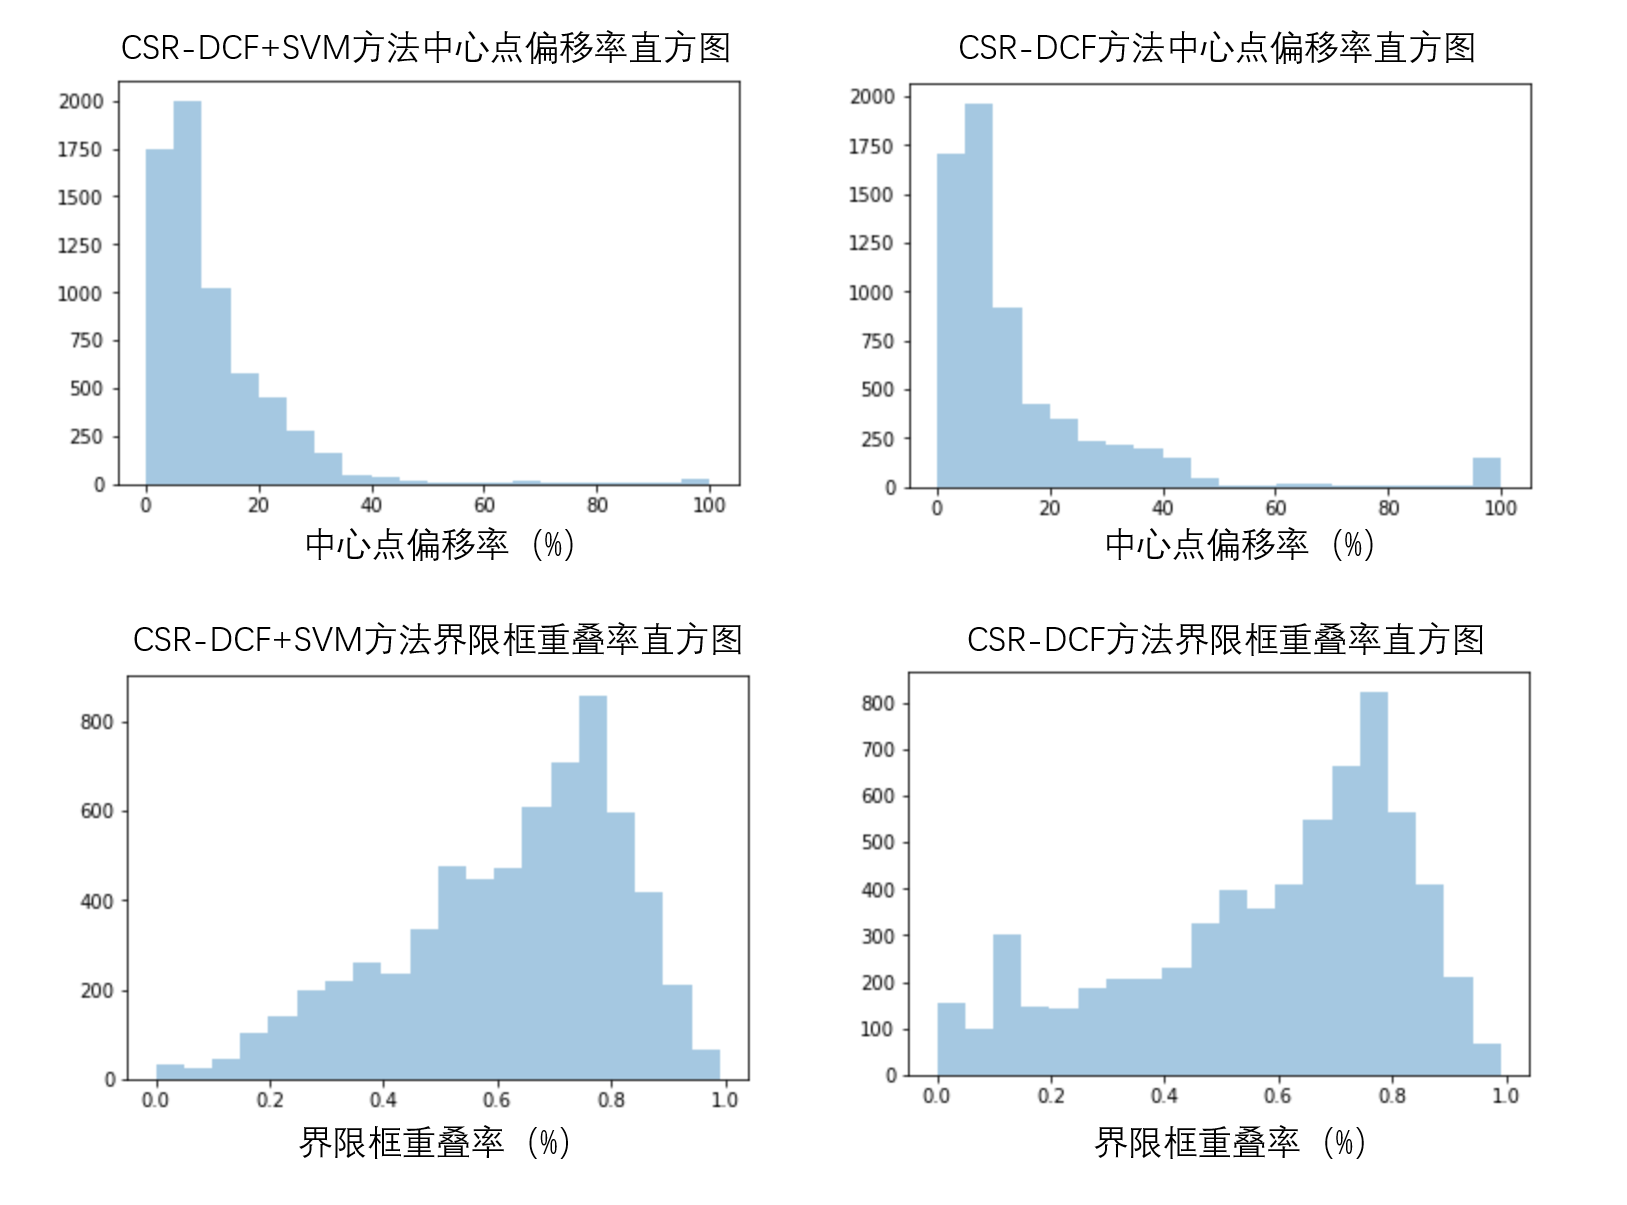
\includegraphics[width=1.0\textwidth]{result-histograms.png}
  \caption{CSR-DCF+SVM系统和CSR-DCF系统结果的中心点偏移率和界限框重叠率统计图}
  \label{fig:resulthistogram}
\end{figure}

  使用目标检测和追踪数据集TB-100\cite{Wu2015Object}中的14个行人追踪视频序列进行测试,这14个视频囊括了包括光照变化、遮挡、目标变形、平面内旋转、平面外旋转、背景相似目标干扰、低分辨率、尺度变化、运动模糊、快速移动、低分辨率这些视频追踪中的常见难点。在测试中,分别统计追踪器得到的界限框与实际的重叠率,即两个界限框重叠区域的大小占它们总面积的比例,以及界限框中心点相对于实际界限框的偏移比例。由于在检测到目标区域后,接下来还会使用该区域的中心点作为目标的坐标控制机器人向其移动,所以使用中心点偏移衡量追踪和识别的精确程度,但由于中心点偏移率无法衡量追踪的尺度是否准确,所以另外引入重叠率。对于14个视频总共6448帧的图像,统计在每一帧上重叠率的平均值和重叠率超过50\%的帧数,以及中心点偏移率的平均值,偏移率超过50\%和20\%的帧数。为了验证加入分类器是否提高了系统准确度,还采用了只使用CSR-DCF追踪器的结果作为比较。

  在6448帧中,CSR-DCF+SVM系统出现了10帧的追踪失败,平均重叠率为62.16\%,有1625帧重叠率小于50\%;由于没有分类器帮助恢复,CSR-DCF系统的追踪失败则为141帧,平均重叠率为58.26\%,有2027帧的重叠率低于50\%。在中心点偏差方面,CSR-DCF+SVM系统的平均中心点偏差率为15.81\%,有108帧偏差率大于50\%,有82.74\%的帧中心点偏差率小于20\%;而CSR-DCF系统则有232帧的中心点偏差量超过50\%,77.73\%的帧中心点偏差率小于20\%,中心点偏差量平均值为27.32\%。具体的分布如图\ref{fig:resulthistogram}所示。



\begin{figure}[htb]
  \centering
  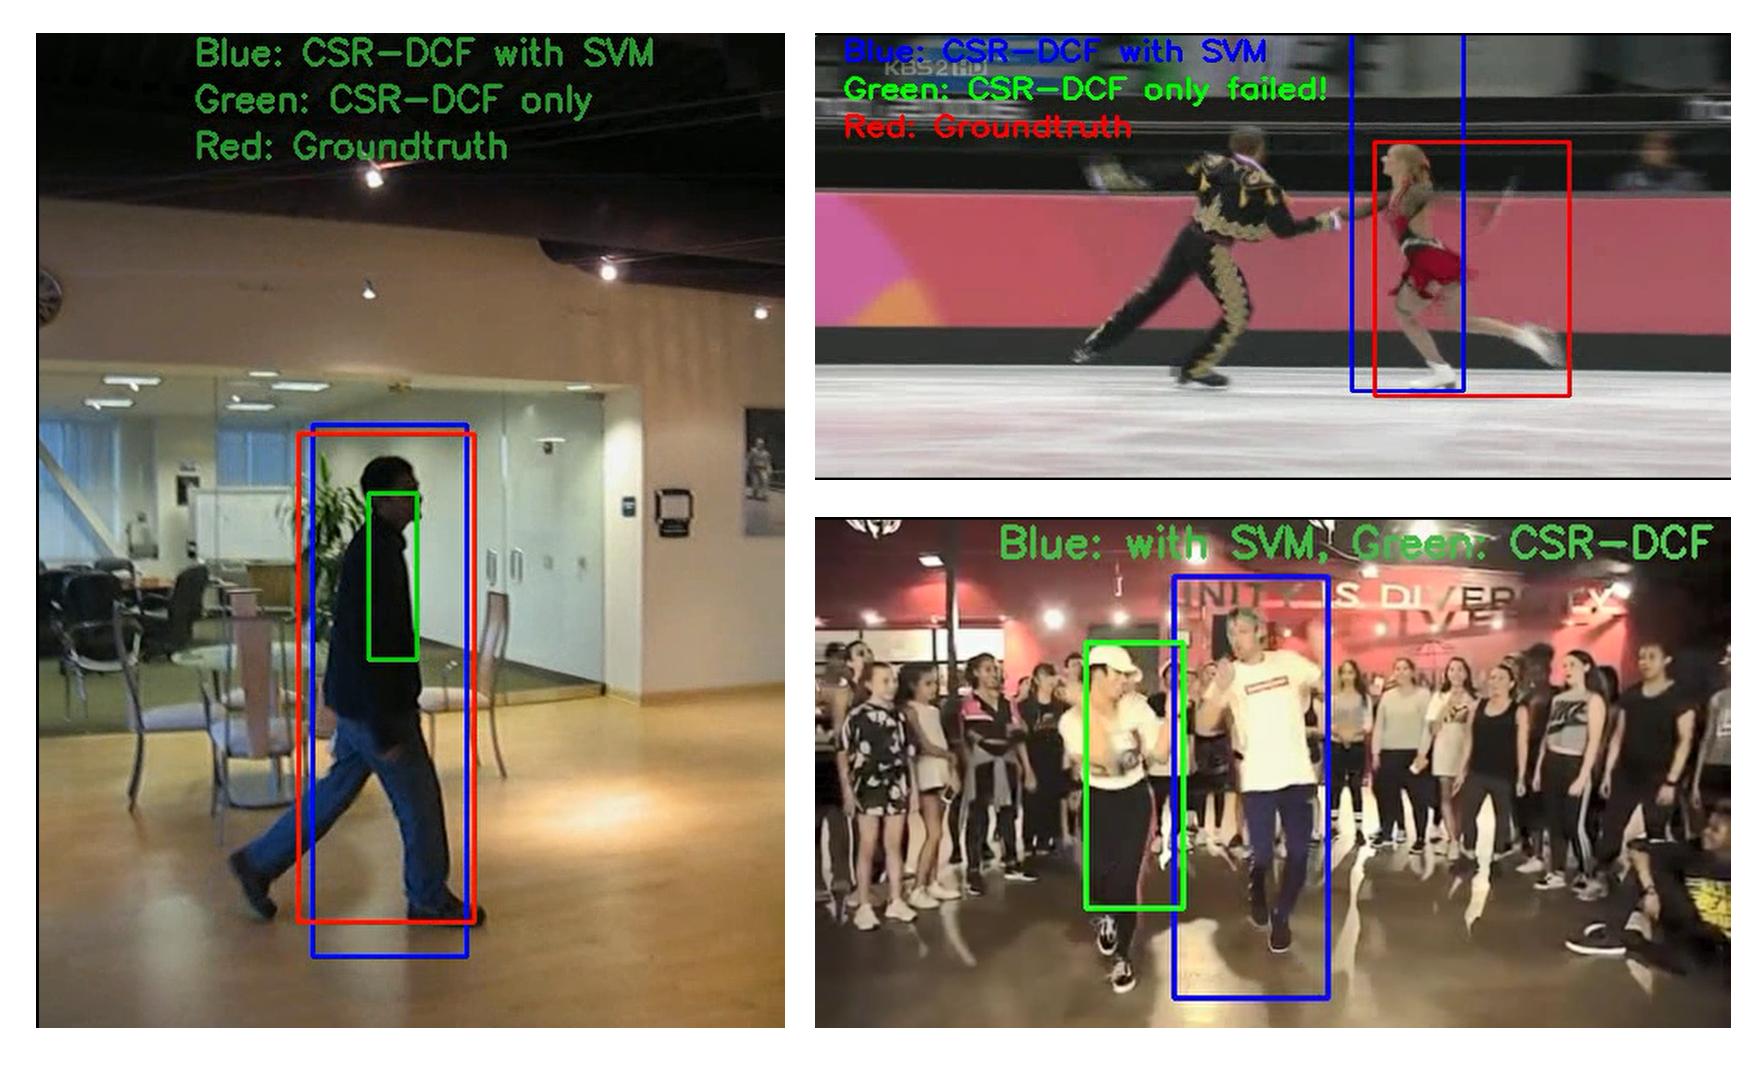
\includegraphics[width=0.8\textwidth]{samples.png}
  \caption{左:由于目标尺度变化导致CSR-DCF追踪器处于错误的尺度上;右上:由于目标运动速度过快导致CSR-DCF算法直接失败;右下:由于目标被另一个人物暂时遮挡导致CSR-DCF算法追踪了错误的行人。}
  \label{fig:samples}
\end{figure}

  实际上,在大部分情况下,由于CSR-DCF算法自身良好的性能,SVM对其的帮助有限,但在复杂情况下追踪失败,或者有遮挡情况下追踪器错误追踪了其他物体,由于尺度变化导致界限框处于错误的尺度等情况时,SVM便能对其提供有效地校正措施。如图\ref{fig:samples}所示。


  在追踪速度方面,在测试的14个视频上,单独使用CSR-DCF可以达到40.78FPS的平均帧率,而加入SVM后,平均帧率降为16.36FPS,勉强能够进行实时的使用。CSR-DCF+SVM系统的帧率收到视频质量的影响较大。当人物未收到遮挡或发生形变较小时,仅使用SVM来进行验证几乎不会影响视频帧率;而当SVM验证错误,或者追踪失败,而导致需要进行全局的扫描检测时,便会大大拖慢整体帧率。
%% !TeX root = ../main.tex

\chapter{浮动体}

\section{三线表}

三线表是《撰写手册》推荐使用的格式,如表~\ref{tab:exampletable}。
\begin{table}[htb]
  \centering\small
  \caption{表号和表题在表的正上方}
  \label{tab:exampletable}
  \begin{tabular}{cl}
    \toprule
    类型   & 描述                                       \\
    \midrule
    挂线表 & 挂线表也称系统表、组织表,用于表现系统结构 \\
    无线表 & 无线表一般用于设备配置单、技术参数列表等   \\
    卡线表 & 卡线表有完全表,不完全表和三线表三种       \\
    \bottomrule
  \end{tabular}
  \note{注:表注分两种,第一种是对全表的注释,用不加阿拉伯数字排在表的下边,
    前面加“注:”;第二种是和表内的某处文字或数字相呼应的注,
    在表里面用带圈的阿拉伯数字在右上角标出,然后在表下面用同样的圈码注出来}
\end{table}

编制表格应简单明了,表达一致,明晰易懂,表文呼应、内容一致。
排版时表格字号略小,或变换字体,尽量不分页,尽量不跨节。
表格太大需要转页是,需要在续表上方注明“续表”,表头页应重复排出。



\section{插图}

有的同学可能听说“\LaTeX{} 只能使用 eps 格式的图片”,甚至把 jpg 格式转为 eps。
事实上,这种做法已经过时。
而且每次编译时都要要调用外部工具解析 eps,导致降低编译速度。
所以我们推荐矢量图直接使用 pdf 格式,位图使用 jpeg 或 png 格式。
\begin{figure}[htb]
  \centering
  
\includegraphics[width=0.3\textwidth]{ustc_logo_fig.pdf}
  \caption{图号、图题置于图的下方}
  \label{fig:logo}
  \note{注:图注的内容不宜放到图题中。}
\end{figure}

关于图片的并排,推荐使用较新的 \pkg{subcaption} 宏包,
不建议使用 \pkg{subfigure} 或 \pkg{subfig} 等宏包。



\section{算法环境}

模板中使用 \pkg{algorithm2e} 宏包实现算法环境。关于该宏包的具体用法,
请阅读宏包的官方文档。

\begin{algorithm}[htb]
  \small
  \SetAlgoLined
  \KwData{this text}
  \KwResult{how to write algorithm with \LaTeX2e }

  initialization\;
  \While{not at end of this document}{
    read current\;
    \eIf{understand}{
      go to next section\;
      current section becomes this one\;
    }{
      go back to the beginning of current section\;
    }
  }
  \caption{算法示例1}
  \label{algo:algorithm1}
\end{algorithm}

注意,我们可以在论文中插入算法,但是插入大段的代码是愚蠢的。
然而这并不妨碍有的同学选择这么做,对于这些同学,建议用 \pkg{listings} 宏包。

%% !TeX root = ../main.tex

\chapter{数学}

\section{数字和单位}

宏包 \pkg{siunitx} 提供了更好的数字和单位支持:
\begin{itemize}
  \item \num{12345.67890}
  \item \num{1+-2i}
  \item \num{.3e45}
  \item \num{1.654 x 2.34 x 3.430}
  \item \si{kg.m.s^{-1}}
  \item \si{\micro\meter} $\si{\micro\meter}$
  \item \si{\ohm} $\si{\ohm}$
  \item \numlist{10;20}
  \item \numlist{10;20;30}
  \item \SIlist{0.13;0.67;0.80}{\milli\metre}
  \item \numrange{10}{20}
  \item \SIrange{10}{20}{\degreeCelsius}
\end{itemize}



\section{数学符号和公式}

\LaTeX{} 默认按照美国的习惯排版数学公式和符号,
但是《撰写手册》要求数学符号依据《GB 3102.11--1993》执行,
与 \LaTeX{} 的习惯有所差异。
本模板基于 \pkg{unicode-math} 配置数学符号,以遵循国标的规定。

注意,\pkg{unicode-math} 宏包与 \pkg{amsfonts}, \pkg{amssymb}, \pkg{bm},
\pkg{mathrsfs}, \pkg{upgreek} 等宏包\emph{不}兼容。
本模板作了处理,用户可以直接使用这些宏包的命令,如 \cs{bm}, \cs{mathscr},
\cs{upGamma}。

本模板中数学符号的用法与 \LaTeX{} 传统有些区别:
\begin{itemize}
  \item 数学常数和特殊函数使用正体,
    如圆周率 $\symup{\pi}$、$\symup{\Gamma}$ 函数。
    应使用 \pkg{unicode-math} 宏包提供的 \cs{symup} 命令转为正体,
    如 \verb|\symup{\pi}|。
  \item 向量和矩阵粗斜体,应使用 \cs{symbf} 命令,
    如 \verb|\symbf{u}|、\verb|\symbf{A}|。
  \item 有限增量符号 $\increment$ (U+2206)应使用 \cs{increment} 命令。
  \item 微分符号 $\dif$ 使用正体,本模板提供了 \cs{dif} 命令。
\end{itemize}

除此之外,模板还提供了一些命令方便使用:
\begin{itemize}
  \item 常数 $\upe$:\verb|\upe|
  \item 负数单位 $\upi$:\verb|\upi|
  \item 圆周率 $\uppi$:\verb|\uppi|
  \item $\argmax$:\verb|\argmax|
  \item $\argmin$:\verb|\argmin|
\end{itemize}

关于数学符号更多的用法,参见 \pkg{unicode-math} 宏包的使用说明和符号列表
\pkg{unimath-symbols}。

在编辑数学公式时,最好避免直接使用字体命令,
而应该定义一些语义命令取代字体命令,
这样输入更简单,也让 \LaTeX{} 代码更有可读性,
而且还方便根据需要统一修改改格式,比如:
\begin{itemize}
  \item 向量 $\vec{x}$:\verb|\renewcommand\vec{\symbf}|
  \item 矩阵 $\mat{A}$:\verb|\newcommand\mat{\symbf}|
  \item 张量 $\ts{T}$: \verb|\newcommand\ts{\symbfsf}|
\end{itemize}

更多的例子:
\begin{equation}
  \upe^{\upi\uppi} + 1 = 0
\end{equation}
\begin{equation}
  \frac{\dif^2 u}{\dif t^2} = \int f(x) \dif x
\end{equation}
\begin{equation}
  \argmin_x f(x)
\end{equation}
\begin{equation}
  \mat{A} \vec{x} = \lambda \vec{x}
\end{equation}



\section{定理和证明}

示例文件中使用 \pkg{amsthm} 宏包配置了定理、引理和证明等环境。
用户也可以使用  \pkg{ntheorem} 宏包。

\begin{definition}
  If the integral of function $f$ is measurable and non-negative, we define
  its (extended) \textbf{Lebesgue integral} by
  \begin{equation}
    \int f = \sup_g \int g,
  \end{equation}
  where the supremum is taken over all measurable functions $g$ such that
  $0 \le g \le f$, and where $g$ is bounded and supported on a set of
  finite measure.
\end{definition}

\begin{assumption}
The communication graph is strongly connected.
\end{assumption}

\begin{example}
  Simple examples of functions on $\real^d$ that are integrable
  (or non-integrable) are given by
  \begin{equation}
    f_a(x) =
    \begin{cases}
      |x|^{-a} & \text{if } |x| \le 1, \\
      0        & \text{if } x > 1.
    \end{cases}
  \end{equation}
  \begin{equation}
    F_a(x) = \frac{1}{1 + |x|^a}, \qquad \text{all } x \in \real^d.
  \end{equation}
  Then $f_a$ is integrable exactly when $a < d$, while $F_a$ is integrable
  exactly when $a > d$.
\end{example}

\begin{lemma}[Fatou]
  Suppose $\{f_n\}$ is a sequence of measurable functions with $f_n \geq 0$.
  If $\lim_{n \to \infty} f_n(x) = f(x)$ for a.e. $x$, then
  \begin{equation}
    \int f \le \liminf_{n \to \infty} \int f_n.
  \end{equation}
\end{lemma}

\begin{remark}
  We do not exclude the cases $\int f = \infty$,
  or $\liminf_{n \to \infty} f_n = \infty$.
\end{remark}

\begin{corollary}
  Suppose $f$ is a non-negative measurable function, and $\{f_n\}$ a sequence
  of non-negative measurable functions with
  $f_n(x) \le f(x)$ and $f_n(x) \to f(x)$ for almost every $x$. Then
  \begin{equation}
    \lim_{n \to \infty} \int f_n = \int f.
  \end{equation}
\end{corollary}

\begin{proposition}
  Suppose $f$ is integrable on $\real^d$. Then for every $\epsilon > 0$:
  \begin{enumerate}
    \renewcommand{\theenumi}{\roman{enumi}}
    \item There exists a set of finite measure $B$ (a ball, for example) such
      that
      \begin{equation}
        \int_{B^c} |f| < \epsilon.
      \end{equation}
    \item There is a $\delta > 0$ such that
      \begin{equation}
        \int_E |f| < \epsilon \qquad \text{whenever } m(E) < \delta.
      \end{equation}
  \end{enumerate}
\end{proposition}

\begin{theorem}
  Suppose $\{f_n\}$ is a sequence of measurable functions such that
  $f_n(x) \to f(x)$ a.e. $x$, as $n$ tends to infinity.
  If $|f_n(x)| \le g(x)$, where $g$ is integrable, then
  \begin{equation}
    \int |f_n - f| \to 0 \qquad \text{as } n \to \infty,
  \end{equation}
  and consequently
  \begin{equation}
    \int f_n \to \int f \qquad \text{as } n \to \infty.
  \end{equation}
\end{theorem}

\begin{proof}
  Trivial.
\end{proof}

\newtheorem*{axiomofchoice}{Axiom of choice}
\begin{axiomofchoice}
  Suppose $E$ is a set and ${E_\alpha}$ is a collection of
  non-empty subsets of $E$. Then there is a function $\alpha
  \mapsto x_\alpha$ (a ``choice function'') such that
  \begin{equation}
    x_\alpha \in E_\alpha,\qquad \text{for all }\alpha.
  \end{equation}
\end{axiomofchoice}

\newtheorem{observation}{Observation}
\begin{observation}
  Suppose a partially ordered set $P$ has the property
  that every chain has an upper bound in $P$. Then the
  set $P$ contains at least one maximal element.
\end{observation}
\begin{proof}[A concise proof]
  Obvious.
\end{proof}

%% !TeX root = ../main.tex

\chapter{引用文献的标注}

模板使用 \pkg{natbib} 宏包来设置参考文献引用的格式,
更多引用方法可以参考该宏包的使用说明。



\section{顺序编码制}

\subsection{角标数字标注法}

\citestyle{super}
\noindent
\begin{tabular}{l@{\quad$\Rightarrow$\quad}l}
  \verb|\cite{knuth86a}|         & \cite{knuth86a}         \\
  \verb|\citet{knuth86a}|        & \citet{knuth86a}        \\
  \verb|\cite[42]{knuth86a}|     & \cite[42]{knuth86a}     \\
  \verb|\cite{knuth86a,tlc2}|    & \cite{knuth86a,tlc2}    \\
  \verb|\cite{knuth86a,knuth84}| & \cite{knuth86a,knuth84} \\
\end{tabular}


\subsection{数字标注法}

\citestyle{numbers}
\noindent
\begin{tabular}{l@{\quad$\Rightarrow$\quad}l}
  \verb|\cite{knuth86a}|         & \cite{knuth86a}         \\
  \verb|\citet{knuth86a}|        & \citet{knuth86a}        \\
  \verb|\cite[42]{knuth86a}|     & \cite[42]{knuth86a}     \\
  \verb|\cite{knuth86a,tlc2}|    & \cite{knuth86a,tlc2}    \\
  \verb|\cite{knuth86a,knuth84}| & \cite{knuth86a,knuth84} \\
\end{tabular}



\section{著者-出版年制标注法}

\citestyle{authoryear}
\noindent
\begin{tabular}{l@{\quad$\Rightarrow$\quad}l}
  \verb|\cite{knuth86a}|         & \cite{knuth86a}         \\
  \verb|\citep{knuth86a}|        & \citep{knuth86a}        \\
  \verb|\cite[42]{knuth86a}|     & \cite[42]{knuth86a}     \\
  \verb|\cite{knuth86a,tlc2}|    & \cite{knuth86a,tlc2}    \\
  \verb|\cite{knuth86a,knuth84}| & \cite{knuth86a,knuth84} \\
\end{tabular}

\vskip 2ex \citestyle{super}
注意,参考文献列表中的每条文献在正文中都要被引用
\cite{slg,lyc,ljs,cgw,cjb,kqy,yhs,yx,dwx,jxz,wjk,syw,wf,xd,twh,huston}。

% !TeX root = ../main.tex

\chapter{总结}

  通过对于已有机器人行人跟随解决方案的调研,本文确定了从视觉行人追踪算法为基础的机器人行人跟随方法。在视觉行人追踪领域,调研了常用的包括卡尔曼滤波、粒子滤波、均值漂移、相关滤波等视觉目标追踪算法,经过实验后,最终选定了相关滤波中的CSR-DCF算法作为本文系统中追踪器的实现算法。CSR-DCF算法对于遮挡、形变、光照都在一定程度上鲁棒,且可以适应目标的尺度变化,是目前视觉追踪中准确度和速度都较为优秀的算法之一。但由于CSR-DCF算法存在对目标失去追踪后难以恢复的问题,且在复杂情况下可能会出现错误的追踪,本文还调研了一系列单帧上的行人检测算法,在深度学习算法和人工特征-分类器算法之间权衡后,选择使用HOG结合HSV直方图作为特征,SVM作为分类器进行行人检测,以防止追踪器发生误判或漏判现象,以及帮助追踪器从追踪失败中进行恢复。

  本文最终实现的视觉行人追踪系统比起仅使用CSR-DCF算法追踪的系统,可以在一定程度上处理追踪器错误追踪其他行人或物体的情况,并且当追踪器失去对目标的追踪后,只要目标回到画面中,便可以很快地恢复追踪。同时,运行速度在大部分时候可以达到实时水平。

  此外,本文还调研了ROS中的导航系统,包括ROS提供的开源导航包和由中国科大研发的可佳导航系统。在使用视觉行人追踪系统得到行人在RGB图像中的位置后,通过对齐Kinect深度图像得到行人在机器人坐标系中的三维位置,设置为目标后再调用导航系统中的导航功能便可以实现稳定的行人跟随系统。
\bibliography{bib/ustc}

%\appendix
%% !TeX root = ../main.tex

\chapter{详细实验结果}



\begin{figure}[htb]
  \centering
  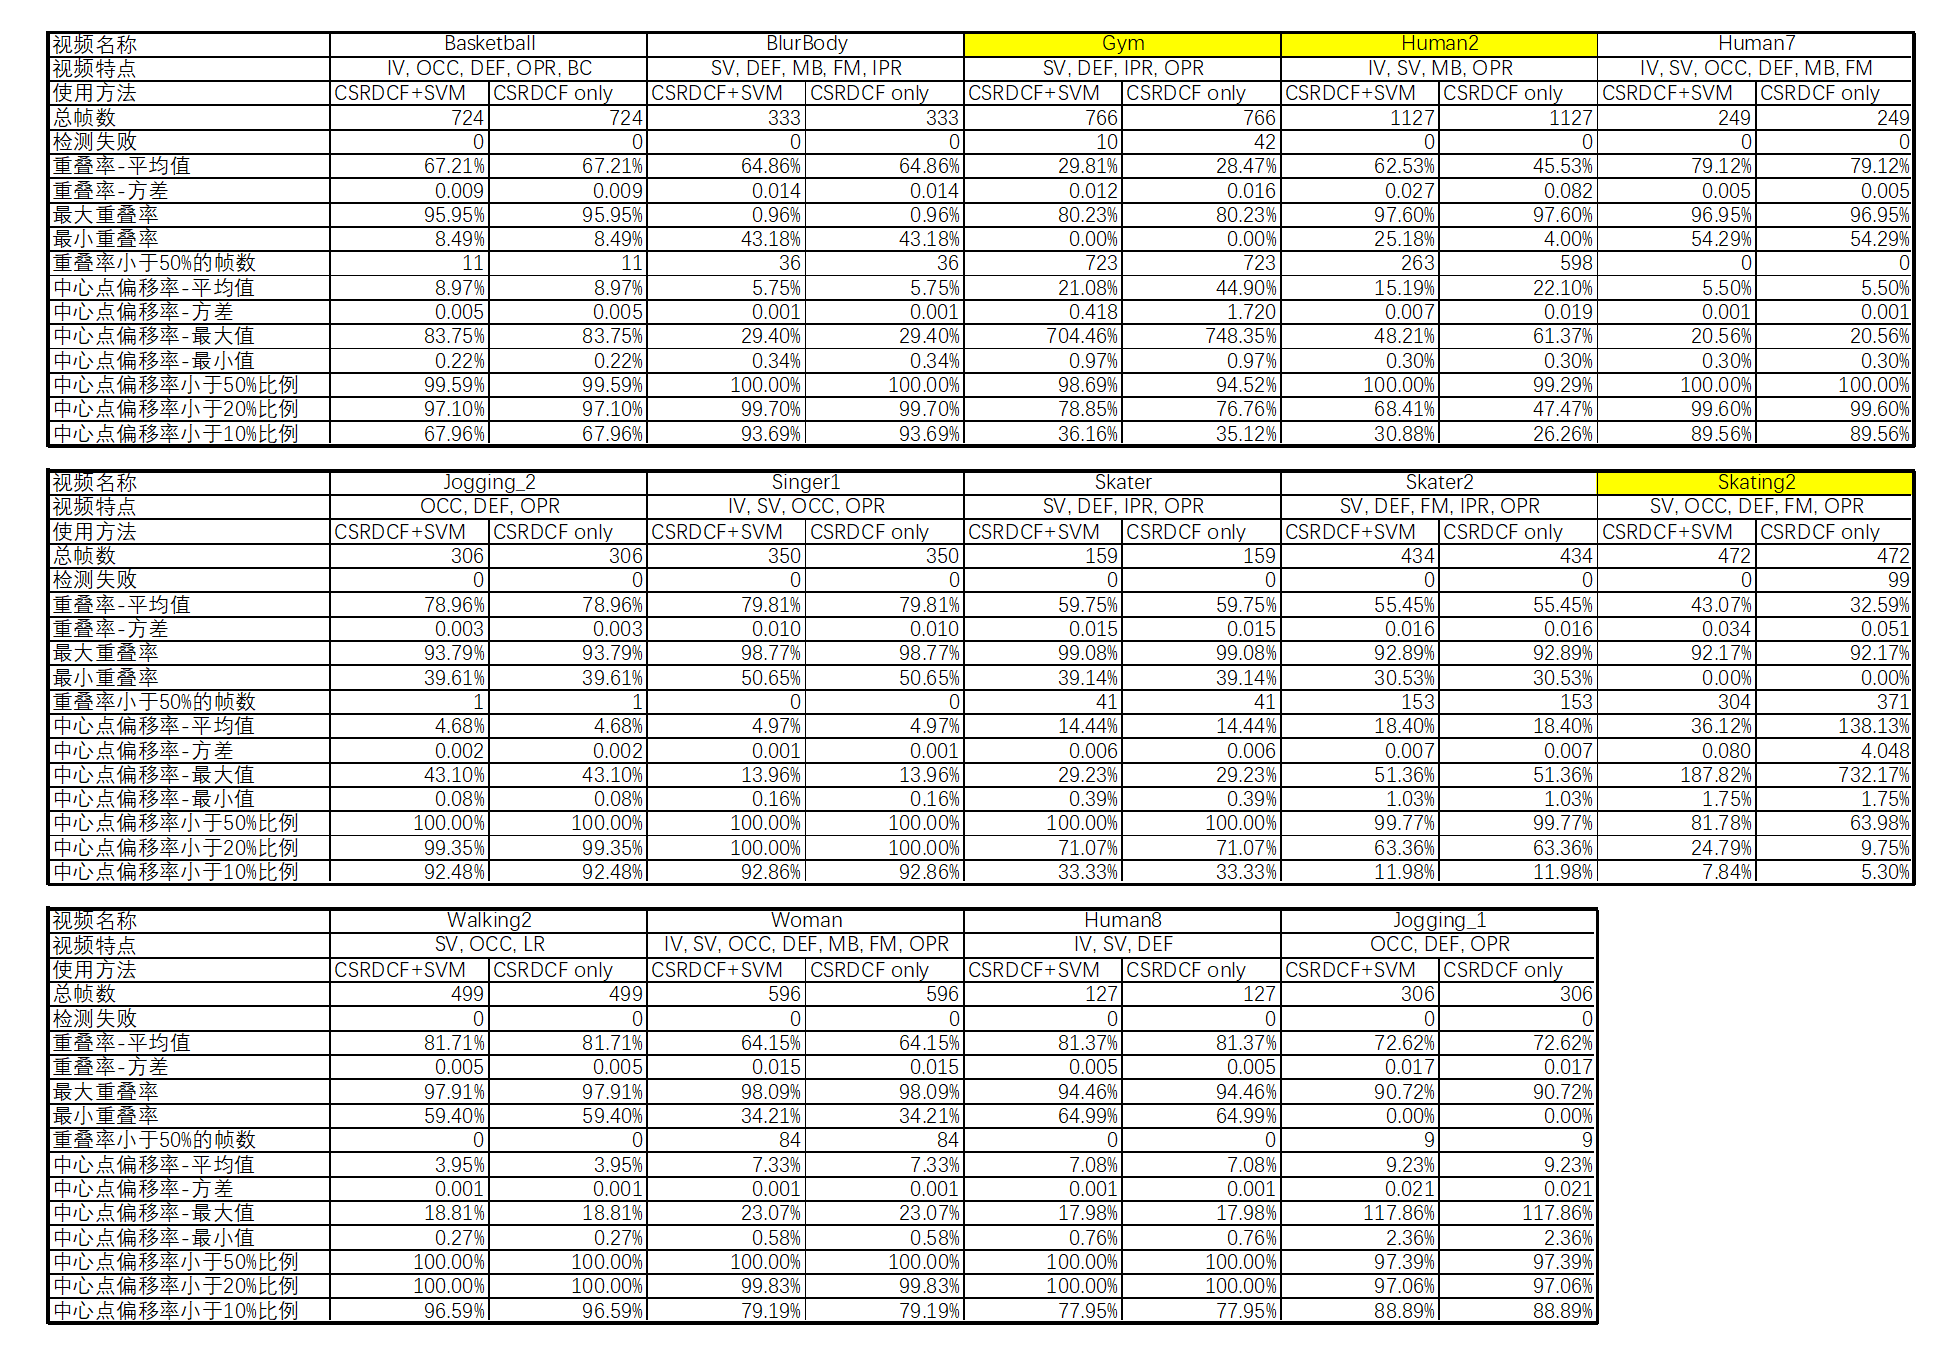
\includegraphics[width=1.1\textwidth]{result.png}
  \caption{详细实验数据}
  \label{fig:results}
\end{figure}




\backmatter
% !TeX root = ../main.tex

\begin{acknowledgements}

在研究学习期间,我有幸得到了三位老师的教导,
他们是:我的导师,中国科大XXX研究员,中科院X昆明动物所马老师以及美国犹他大学的XXX老师。
三位深厚的学术功底,严谨的工作态度和敏锐的科学洞察力使我受益良多。
衷心感谢他们多年来给予我的悉心教导和热情帮助。

感谢XXX老师在实验方面的指导以及教授的帮助。
科大的XXX同学和XXX同学参与了部分试验工作,在此深表谢意。

\end{acknowledgements}

%% !TeX root = ../main.tex

\begin{publications}

\section*{已发表论文}

\begin{enumerate}
\item A A A A A A A A A
\item A A A A A A A A A
\item A A A A A A A A A
\end{enumerate}

\section*{待发表论文}

\begin{enumerate}
\item A A A A A A A A A
\item A A A A A A A A A
\item A A A A A A A A A
\end{enumerate}

\section*{研究报告}
\begin{enumerate}
\item A A A A A A A A A
\item A A A A A A A A A
\item A A A A A A A A A
\end{enumerate}

\end{publications}


\end{document}
